% ============================================================
% Báo cáo giữa kỳ — Học máy trên đồ thị
% Phần A: GraphVis (seminar) — Phần B: SciMKG (chỉ báo cáo)
% Biên dịch: xelatex main -> bibtex main -> xelatex main x2
%   (hoặc: latexmk -xelatex main)
% ============================================================
\documentclass[conference]{IEEEtran}
\IEEEoverridecommandlockouts

% ---------- Ngôn ngữ & phông ----------
\usepackage{fontspec}
\setmainfont{Times New Roman}[NFSSFamily=ptm]
\setmonofont{Consolas}[Scale=0.85]
\usepackage[vietnamese]{babel}

% ---------- Gói chung ----------
\usepackage{cite}
\usepackage{amsmath,amssymb,amsfonts}
\usepackage{algorithmic}
\usepackage{graphicx}
\usepackage{textcomp}
\usepackage[table]{xcolor}
\usepackage{booktabs}
\usepackage{multirow}
\usepackage{makecell}
\usepackage{tikz}
\usetikzlibrary{arrows.meta,positioning,fit,backgrounds,calc,shapes.geometric}
\usepackage[hidelinks]{hyperref}
\usepackage{url}

% ---------- Đổi tên thành phần IEEE sang tiếng Việt ----------
\addto\captionsvietnamese{%
  \renewcommand{\abstractname}{Tóm tắt}%
  \renewcommand{\figurename}{Hình}%
  \renewcommand{\tablename}{Bảng}%
  \renewcommand{\refname}{Tài liệu tham khảo}%
}
\renewcommand{\IEEEkeywordsname}{Từ khóa}
% Từ khóa của algorithmic
\renewcommand{\algorithmicrequire}{\textbf{Vào:}}
\renewcommand{\algorithmicensure}{\textbf{Ra:}}
\renewcommand{\algorithmicfor}{\textbf{với}}
\renewcommand{\algorithmicdo}{\textbf{làm}}
\renewcommand{\algorithmicend}{\textbf{hết}}

% ---------- Macro tiện ích ----------
% Đánh dấu việc còn phải làm (xóa hết trước khi nộp: grep "\\todo")
\newcommand{\todo}[1]{\textcolor{red}{\textbf{[TODO:} #1\textbf{]}}}
% Link W&B công khai cho từng thực nghiệm
\newcommand{\wandb}[1]{\textcolor{blue}{\textbf{W\&B:} \url{#1}}}
\newcommand{\wandbtodo}{\textcolor{blue}{\textbf{W\&B:}} \todo{link báo cáo W\&B công khai}}
% Tiêu đề phân phần (Phần A / Phần B)
\newcommand{\phan}[2]{%
  \vspace{6pt}\noindent\colorbox{black!8}{\parbox{\dimexpr\columnwidth-2\fboxsep}{%
  \centering\large\bfseries #1\\[1pt]\normalsize\mdseries\itshape #2}}\vspace{2pt}}
\newcommand{\GV}{\textsc{GraphVis}}
\newcommand{\SM}{\textsc{SciMKG}}
\newcommand{\Dg}{\mathcal{D}_g}
\newcommand{\Dv}{\mathcal{D}_v}

\begin{document}

% ---------- Trang bìa ----------
% Trang bìa (một cột) — tính vào giới hạn 25 trang
\begin{titlepage}
\centering
{\large ĐẠI HỌC QUỐC GIA THÀNH PHỐ HỒ CHÍ MINH\par}
{\large\bfseries TRƯỜNG ĐẠI HỌC KHOA HỌC TỰ NHIÊN\par}
{\large KHOA CÔNG NGHỆ THÔNG TIN\par}
\vspace{1.2cm}

\includegraphics[width=4.2cm]{figures/logo_hcmus.pdf}\par
\vspace{1.2cm}
{\Large\bfseries BÁO CÁO GIỮA KỲ\par}
\vspace{0.3cm}
{\large Môn học: Học máy trên đồ thị\par}
\vspace{1.0cm}
{\LARGE\bfseries BÁO CÁO HAI MÔ HÌNH:\par GraphVis và SciMKG\par}
\vspace{1.0cm}
\begin{tabular}{ll}
\textbf{Bài seminar:} & GraphVis: Boosting LLMs with Visual Knowledge Graph Integration \\
                      & (NeurIPS 2024) \\[4pt]
\textbf{Bài báo cáo:} & SciMKG: A Multimodal Knowledge Graph for Science Education \\
                      & with Text, Image, Video and Audio (AAAI 2026)
\end{tabular}
\vfill
\begin{tabular}{ll}
\textbf{Giảng viên:} & Lê Ngọc Thành \\[4pt]
\textbf{Học viên:}   & Âu Dương Khang - 25C15045 \\
                     & Nguyễn Bùi Mẫn Nhi - 25C15055 \\[4pt]
\textbf{Mã nguồn:}   & \url{https://github.com/AuDuongKhang/graphml-seminar-report} \\
\textbf{W\&B:}       & năm báo cáo công khai, liệt kê ở Phụ lục~\ref{app:links}
\end{tabular}
\vspace{1.5cm}

{\large TP. Hồ Chí Minh, tháng 10 năm 2026\par}
\end{titlepage}


% ---------- Tiêu đề bài ----------
\title{Báo cáo hai mô hình: GraphVis và SciMKG}

\author{\IEEEauthorblockN{Âu Dương Khang}
\IEEEauthorblockA{\textit{MSHV: 25C15045}\\
Trường ĐH Khoa học Tự nhiên, ĐHQG-HCM}
\and
\IEEEauthorblockN{Nguyễn Bùi Mẫn Nhi}
\IEEEauthorblockA{\textit{MSHV: 25C15055}\\
Trường ĐH Khoa học Tự nhiên, ĐHQG-HCM}
}

\maketitle

\begin{abstract}
\todo{Viết sau cùng (150--200 từ): giới thiệu ngắn hai bài (GraphVis: đưa đồ thị con dạng ảnh vào LVLM, huấn luyện hai giai đoạn; SciMKG: dựng tự động đồ thị tri thức giáo dục đa phương thức bằng nhiều LLM); điều nhóm làm được: trình bày chi tiết cơ chế hoạt động, đối chiếu bài báo với mã nguồn, phân tích ảnh hưởng độ phức tạp ảnh, tái lập thực nghiệm và các phát hiện chính.}
\end{abstract}

\begin{IEEEkeywords}
đồ thị tri thức, mô hình ngôn ngữ--thị giác lớn, học theo giáo trình, đồ thị tri thức đa phương thức, trích xuất khái niệm
\end{IEEEkeywords}

% ============================================================
% I. GIỚI THIỆU  (~0,7 trang) — SƯỜN, viết sau Phần A/B
% Hai bài được chọn độc lập, KHÔNG cần ép liên kết.
% ============================================================
\section{Giới thiệu}\label{sec:intro}

\todo{Viết đoạn văn hoàn chỉnh theo các ý dưới.}

% Ý 1 — Bối cảnh chung ngắn gọn: đồ thị tri thức (KG) là cách biểu diễn tri thức có cấu trúc;
%       LLM/LVLM hiện nay vừa có thể dùng KG, vừa có thể giúp xây KG.
% Ý 2 — Bài thứ nhất (seminar): GraphVis [deng2024graphvis] — bài toán QA thường thức có KG hỗ trợ;
%       ý tưởng vẽ đồ thị con thành ảnh cho LVLM; huấn luyện hai giai đoạn. -> Phần A.
% Ý 3 — Bài thứ hai: SciMKG [lu2026scimkg] — dựng tự động KG giáo dục K12 với văn bản, ảnh,
%       video, âm thanh bằng chuỗi nhiều LLM (EVIA) và căn chỉnh đa phương thức. -> Phần B.
% Ý 4 — Nội dung báo cáo (gạch đầu dòng):
%       - trình bày chi tiết cơ chế hoạt động của từng hệ thống (dữ liệu vào/ra, mô hình dùng ở mỗi bước,
%         cách huấn luyện hoặc cách gọi mô hình), đối chiếu bài báo với mã nguồn công bố;
%       - phân tích ảnh hưởng của kích thước/độ phân giải ảnh đồ thị lên GraphVis;
%       - tái lập thực nghiệm của cả hai bài, log W&B công khai;
%       - nhận xét về tính nhất quán số liệu và khả năng tái lập.
% Ý 5 — Cấu trúc báo cáo: II nền tảng; III–VIII GraphVis; IX–XIII SciMKG; XIV kết luận.

% ============================================================
% II. KIẾN THỨC NỀN  (~1,5 trang) — SƯỜN
% Chỉ trình bày những gì hai phần sau thực sự dùng.
% ============================================================
\section{Kiến thức nền}\label{sec:background}

\subsection{Đồ thị tri thức và ConceptNet}
\todo{Định nghĩa KG $\mathcal{G}=(\mathcal{V},\mathcal{E})$ với bộ ba (đầu, quan hệ, đuôi); KG thường thức vs KG thực thể; ConceptNet 5.5: nút là khái niệm đời thường, cạnh có hướng và nhãn; bản tiếng Anh dùng trong GraphVis có 799.273 nút, 2.487.810 cạnh, 42 quan hệ gộp còn 17.}

\subsection{Mô hình ngôn ngữ sinh và tinh chỉnh có giám sát}
\todo{Phân rã tự hồi quy $p_\theta(\mathbf{y}\mid\mathbf{x})=\prod_t p_\theta(y_t\mid\mathbf{x},\mathbf{y}_{<t})$; hàm mất mát NLL của SFT (sẽ dùng lại ở \eqref{eq:gv-loss}); giải mã tham lam khi đánh giá.}

\subsection{Mô hình ngôn ngữ--thị giác lớn (LVLM)}
\todo{Cấu trúc LLaVA: bộ mã hóa ảnh CLIP ViT-L/14 $f_v$, bộ chiếu $f_p$, LLM; ảnh được biến thành chuỗi token thị giác ghép trước token văn bản; LLaVA-1.6 (LLaVA-NeXT) dùng AnyRes khi suy luận. Hình nhỏ vẽ luồng ảnh $\rightarrow$ token.}

\subsection{LoRA}
\todo{$W=W_0+\frac{\alpha}{r}BA$, $B\in\mathbb{R}^{d\times r}$, $A\in\mathbb{R}^{r\times k}$, $r\ll\min(d,k)$; chỉ cập nhật $A,B$; QLoRA (lượng tử hóa 4-bit $W_0$) — phương án nhóm dùng khi tái lập trên Colab nếu bộ nhớ không đủ.}

\subsection{Học theo giáo trình (curriculum learning)}
\todo{Ý tưởng của Bengio và cộng sự: sắp xếp dữ liệu/tác vụ từ dễ đến khó; trong GraphVis ``giáo trình'' ở mức tác vụ (đọc hình $\rightarrow$ trả lời câu hỏi), không phải mức mẫu.}

\subsection{LLM cho trích xuất thông tin}
\todo{NER bằng LLM (GPT-NER, UniversalNER); Self-Refine (vòng phản hồi--sửa); Self-Consistency (bỏ phiếu nhiều lần sinh); các chỉ số Precision/Recall/F1, MCC, AUC; điểm căn chỉnh ảnh--văn bản CLIPScore, BLIP-ITM.}


% ================= PHẦN A =================
\phan{PHẦN A --- GraphVis}{Tăng cường LLM bằng đồ thị tri thức dạng ảnh (NeurIPS 2024)}
% ============================================================
% PHẦN A — GRAPHVIS (bài seminar)   ~ 10 trang
%   I–II Giới thiệu và kiến thức nền riêng (A_intro, A_background)
%   III  Bài toán & động cơ
%   IV   Phương pháp (IV-E: chi tiết huấn luyện)
%   V    Kết quả công bố
%   VI   Độ phức tạp ảnh đồ thị
%   VII  Tái lập (chưa có số liệu)
%   VIII Đánh giá phê bình
%   IX   Kết luận riêng (A_conclusion)
% ============================================================

% ------------------------------------------------------------
\section{GraphVis: bài toán và động cơ}\label{sec:gv-problem}
% ------------------------------------------------------------

\subsection{Vì sao cần đồ thị tri thức}
LLM trả lời trôi chảy nhưng có ba điểm yếu: tự tạo ra thông tin không có thật (ảo giác), nhớ sai tri thức đã học, và muốn cập nhật tri thức thì phải huấn luyện lại với chi phí lớn. Một cách khắc phục là cung cấp tri thức từ bên ngoài ngay lúc suy luận. \GV{}~\cite{deng2024graphvis} chọn nguồn tri thức là ConceptNet~\cite{speer2017conceptnet} vì các tập dữ liệu đánh giá là câu hỏi thường thức (CommonsenseQA~\cite{talmor2019csqa}, OpenBookQA~\cite{mihaylov2018obqa}). Tri thức thường thức hiếm khi được viết thành văn bản vì ai cũng biết, ví dụ ``ngân hàng thường có cửa xoay''. Vì vậy loại tri thức này phải được gom thủ công thành các cặp khái niệm nối với nhau, và kết quả là một đồ thị.

Bản ConceptNet tiếng Anh dùng trong bài có 799.273 nút và 2.487.810 cạnh. Không thể đưa toàn bộ đồ thị vào cửa sổ ngữ cảnh của mô hình, nên mọi phương pháp đều phải trích một đồ thị con liên quan đến câu hỏi trước.

\subsection{Phát biểu bài toán}
Gọi $\mathcal{G}=(\mathcal{V},\mathcal{E})$ là đồ thị tri thức, $\mathbf{x}$ là câu hỏi (kèm các lựa chọn) và $\mathbf{y}$ là đáp án đúng. Gọi $\mathcal{V}_\mathbf{x}\subseteq\mathcal{V}$ là các khái niệm xuất hiện trong câu hỏi và các lựa chọn. Bài toán LLM tăng cường bằng KG gồm hai bước:
\begin{enumerate}
\item \emph{Truy hồi}: một hàm $f$ trả về đồ thị con liên quan
\begin{equation}
\mathcal{G}_\mathbf{x}=f(\mathbf{x},\mathcal{V}_\mathbf{x},\mathcal{G})=(\mathcal{V}_\mathbf{x}',\mathcal{E}_\mathbf{x})\subseteq\mathcal{G}.
\end{equation}
\item \emph{Đưa tri thức vào mô hình}: một hàm $g$ biến $\mathcal{G}_\mathbf{x}$ thành đầu vào mà mô hình dùng được, tạo prompt mở rộng $\mathbf{x}_g=[g(\mathcal{G}_\mathbf{x}),\mathbf{x}]$. Mục tiêu là chọn $g$ sao cho xác suất mô hình sinh ra đáp án đúng, $p_\theta(\mathbf{y}\mid\mathbf{x}_g)$, là lớn nhất.
\end{enumerate}
\GV{} không đề xuất $f$ mới. Bài dùng lại cách truy hồi các đường đi tối đa $k$ bước nối các khái niệm trong $\mathcal{V}_\mathbf{x}$ của MHGRN~\cite{feng2020mhgrn}, với $k=2$. Đóng góp của bài nằm ở cách chọn $g$.

\subsection{Hai hướng chọn $g$ trước đây và đánh đổi giữa chúng}
\textbf{Tuyến tính hóa (linearize).} Viết đồ thị con thành danh sách bộ ba $(h,r,t)$ (đầu, quan hệ, đuôi) rồi chèn vào prompt; KAPING~\cite{baek2023kaping} là ví dụ tiêu biểu. Cách này đơn giản và không phải sửa mô hình. Tuy nhiên, cấu trúc đồ thị bị duỗi thành một chuỗi: muốn biết nút nào là trung tâm, mô hình phải tự ghép lại từ nhiều bộ ba rời rạc. Ngữ cảnh cũng dài thêm. Trên LLaVA-1.6, KAPING làm độ chính xác CSQA giảm từ 70,5\% xuống 67,7\%.

\textbf{Dựa trên GNN.} Mã hóa đồ thị con bằng một GNN rồi chiếu vector biểu diễn sang không gian token của LLM, như QA-GNN~\cite{yasunaga2021qagnn}, GreaseLM~\cite{zhang2022greaselm} và GNP~\cite{tian2024gnp}. Cấu trúc được giữ lại, nhưng LLM không hiểu sẵn loại tín hiệu này. Cần huấn luyện thêm bộ mã hóa và bộ chiếu cho từng tác vụ, và kết quả khó chuyển sang tác vụ khác.

Tóm lại, hướng thứ nhất giữ được khả năng đọc của LLM nhưng làm mất cấu trúc, còn hướng thứ hai giữ cấu trúc nhưng LLM không đọc được ngay. \GV{} đi theo hướng thứ ba: vẽ đồ thị con thành ảnh. Ảnh giữ nguyên bố cục hai chiều của đồ thị, và LVLM vốn đã có sẵn đường xử lý ảnh nên không phải thiết kế thêm mô-đun mới. Bù lại, LVLM chưa quen đọc ảnh đồ thị, nên bài phải dạy mô hình đọc trước khi dùng ảnh để suy luận.

% ------------------------------------------------------------
\section{GraphVis: phương pháp}\label{sec:gv-method}
% ------------------------------------------------------------
Hình~\ref{fig:gv-pipeline} tóm tắt toàn bộ quy trình. Quy trình có hai phần: dựng dữ liệu (đồ thị con $\rightarrow$ ảnh $\rightarrow$ hai tập dữ liệu) và huấn luyện hai giai đoạn trên cùng một LVLM.

\begin{figure*}[t]
\centering
% Quy trình GraphVis: dựng dữ liệu + huấn luyện hai giai đoạn (2 cột, ~16 cm)
\begin{tikzpicture}[
  font=\footnotesize, >={Stealth[length=1.8mm]},
  box/.style={draw, rounded corners=2pt, align=center, inner sep=3pt, minimum height=10mm},
  data/.style={box, fill=yellow!15},
  ds/.style={box, fill=green!12, text width=50mm},
  model/.style={box, fill=black!8, text width=15mm},
  stage/.style={box, fill=orange!20, draw=orange!70!black, text width=32mm},
  lab/.style={font=\scriptsize\itshape, inner sep=1pt},
]
% --- Hàng 1: từ câu hỏi đến ảnh
\node[data, text width=33mm] (q)   at (1.9,0)  {\textbf{Câu hỏi QA} $\mathbf{x}^{(i)}$, đáp án $\mathbf{y}^{(i)}$\\\scriptsize ``Cửa xoay\dots{} biện pháp an ninh ở đâu?''};
\node[box, text width=24mm]  (ret) at (5.6,0)  {Truy hồi $f$\\\scriptsize đường đi $\le$2 bước, ConceptNet};
\node[box, text width=20mm]  (gv)  at (8.7,0)  {Graphviz\\\scriptsize vẽ, không tham số};
\node[data, text width=14mm] (img) at (11.3,0) {ảnh $v^{(i)}$};
\draw[->] (q) -- (ret);
\draw[->] (ret) -- node[above, lab]{$\mathcal{G}_{\mathbf{x}}$} (gv);
\draw[->] (gv) -- (img);

% --- Hàng 2: hai tập dữ liệu từ cùng một ảnh
\node[ds] (dg) at (5.0,-1.75)  {$\Dg=\{(v^{(i)},p_j,a_j)\}_{j=1}^{6}$\\\scriptsize câu hỏi về chính đồ thị; $a_j$ tính tự động từ $\mathcal{G}_{\mathbf{x}}$};
\node[ds] (dv) at (11.3,-1.75) {$\Dv=\{(v^{(i)},\mathbf{x}^{(i)},\mathbf{y}^{(i)})\}$\\\scriptsize câu hỏi QA gốc trong khuôn prompt; đáp án gốc};
\draw[->] (img) -- (dv);
\draw[->] (img.south) -- ++(0,-0.3) -| (dg.north);

% --- Hàng 3: huấn luyện theo giáo trình
\node[model] (m0) at (1.4,-3.6)  {LLaVA-1.6\\ $\theta_0$};
\node[stage] (s1) at (5.0,-3.6)  {\textbf{Giai đoạn 1}: học đọc ảnh\\\scriptsize SFT trên $\Dg$, 1 epoch};
\node[model, text width=9mm] (m1) at (8.15,-3.6) {$\theta_1$};
\node[stage] (s2) at (11.3,-3.6) {\textbf{Giai đoạn 2}: học trả lời\\\scriptsize SFT trên $\Dv$, 1 epoch, khởi tạo từ $\theta_1$};
\node[model] (m2) at (14.9,-3.6) {\GV{}\\ $\theta_2$};
\draw[->] (m0) -- (s1);
\draw[->] (s1) -- (m1);
\draw[->] (m1) -- (s2);
\draw[->] (s2) -- (m2);
\draw[->, dashed] (dg) -- (s1);
\draw[->, dashed] (dv) -- (s2);

\begin{scope}[on background layer]
\node[draw=black!30, dashed, rounded corners, fit=(q)(img)(dg)(dv), inner sep=2mm,
      label={[lab]above right:Phần 1: dựng dữ liệu (lặp với mọi câu hỏi $i$)}] {};
\node[draw=black!30, dashed, rounded corners, fit=(m0)(m2), inner sep=2mm,
      label={[lab]below:Phần 2: huấn luyện theo giáo trình (cùng kiến trúc, cùng hàm mất mát, chỉ khác dữ liệu)}] {};
\end{scope}
\end{tikzpicture}

\caption{Quy trình \GV{} (nhóm vẽ lại).\textbf{Trên}: mỗi câu hỏi QA được truy hồi đồ thị con 2 bước trên ConceptNet và vẽ bằng Graphviz. Cùng một ảnh $v$ tạo ra hai loại mẫu: $\Dg$ gồm câu hỏi về chính đồ thị, với đáp án tính tự động; $\Dv$ gồm câu hỏi QA gốc và đáp án gốc. \textbf{Dưới}: giai đoạn~1 tinh chỉnh trên $\Dg$ và cho ra $\theta_1$; giai đoạn~2 khởi tạo từ $\theta_1$ rồi tinh chỉnh trên $\Dv$ và cho ra $\theta_2$. Hai giai đoạn dùng cùng một kiến trúc và cùng một hàm mất mát, chỉ khác dữ liệu.}
\label{fig:gv-pipeline}
\end{figure*}

\subsection{Truy hồi và trực quan hóa đồ thị con}
Với mỗi câu hỏi, các khái niệm trong câu hỏi và trong từng lựa chọn được khớp với nút ConceptNet. Sau đó hệ thống lấy mọi đường đi dài tối đa hai cạnh nối chúng. 42 loại quan hệ gốc được gộp còn 17 loại (ví dụ \texttt{at location}, \texttt{used for}, \texttt{is a}). Đồ thị con được vẽ bằng Graphviz~\cite{gansner2000graphviz}, một công cụ bố trí đồ thị theo luật, không có tham số học. Ảnh thu được có nút là nhãn khái niệm và cạnh có hướng mang nhãn quan hệ. Trên CSQA, theo ước lượng từ biểu đồ (Hình~4--5 trong~\cite{deng2024graphvis}), phần lớn đồ thị con có khoảng 10--30 nút, nhưng phân bố có đuôi dài tới khoảng 80 nút và 160 cạnh. Đặc điểm này quan trọng cho Mục~\ref{sec:gv-complexity}.

\subsection{Ảnh đồ thị đi vào LVLM như thế nào}
Mô hình gốc là LLaVA-v1.6-Mistral-7B~\cite{liu2024llavanext}, gồm ba khối: bộ mã hóa ảnh $f_v$ (CLIP ViT-L/14, 336\,px~\cite{radford2021clip}), bộ chiếu $f_p$ (MLP hai lớp với GELU) và LLM Mistral-7B~\cite{jiang2023mistral}. Ảnh $e$ được biến thành chuỗi token thị giác $\mathbf{v}=f_p(f_v(e))=[v_1,\dots,v_n]$ cùng số chiều với token chữ, rồi được ghép trước câu hỏi. Xác suất sinh đáp án có dạng
\begin{equation}
p_\theta(\mathbf{y}\mid\mathbf{v},\mathbf{x})=\prod_{j=1}^{m}p_\theta(y_j\mid\mathbf{v},\mathbf{x},\mathbf{y}_{<j}).\label{eq:gv-lvlm}
\end{equation}
Như vậy $g(\mathcal{G}_\mathbf{x})=f_p(f_v(\textsc{Graphviz}(\mathcal{G}_\mathbf{x})))$. Hàm $g$ là ghép của một bước vẽ cố định với hai khối mạng có sẵn trong LVLM.

\subsection{Giai đoạn 1: học đọc ảnh đồ thị}
Khi chưa tinh chỉnh, LLaVA gần như không đọc được ảnh đồ thị. Với yêu cầu liệt kê bộ ba, mô hình trả lời đúng khuôn dạng nhưng nội dung sai hẳn, chẳng hạn ``(node1, node2, node3)''. Độ chính xác khớp tuyệt đối chỉ đạt 0,6\% (Bảng~\ref{tab:gv-reading}). Vì vậy bài tạo tập $\Dg$ gồm sáu tác vụ. Đáp án của mọi tác vụ được tính trực tiếp từ $\mathcal{G}_\mathbf{x}$ nên không cần gán nhãn thủ công:
\begin{itemize}
\item \emph{Nhóm OCR}: (1) liệt kê tên mọi nút; (2) liệt kê mọi bộ ba (đầu, quan hệ, đuôi).
\item \emph{Nhóm cấu trúc}: (3) bậc của một nút cho trước; (4) nút có bậc cao nhất và bậc của nó; (5) đếm số nút; (6) đếm số cạnh.
\end{itemize}
Mỗi tác vụ có năm mẫu câu hỏi diễn đạt khác nhau, và mỗi mẫu dữ liệu chọn ngẫu nhiên một mẫu câu để tăng độ đa dạng. Mỗi ảnh sinh ra một mẫu cho mỗi tác vụ, tức $M=6$ mẫu $(v,p_j,a_j)$.

\subsection{Giai đoạn 2: học trả lời câu hỏi có ảnh hỗ trợ}
Tập $\Dv$ ghép ảnh $v$ với câu hỏi QA gốc theo khuôn:
\begin{quote}\small\ttfamily
<ảnh> The image represents a knowledge graph relevant to the question, which may or may not be useful. Question: <câu hỏi gốc>
\end{quote}
Đáp án giữ nguyên nhãn của tập QA. Khuôn prompt nói rõ rằng ảnh ``có thể có ích hoặc không''. Lý do là đồ thị con truy hồi theo luật có thể thiếu thông tin hoặc chứa nhiễu, nên mô hình phải học cách tự quyết định có dựa vào ảnh hay không.

\subsection{Chi tiết huấn luyện}\label{sec:gv-training}
Hình~\ref{fig:gv-pipeline} cho biết thứ tự hai giai đoạn. Mục này đi sâu vào cách mỗi giai đoạn thực sự được huấn luyện: tối ưu hàm mục tiêu nào, phần nào của mô hình được cập nhật, và với cấu hình nào. Thông tin lấy từ bài báo (Phụ lục~A của~\cite{deng2024graphvis}) và được nhóm đối chiếu với mã nguồn công bố (\texttt{llava/train/train.py}, \texttt{scripts/finetune\_lora.sh}).

\textbf{(a) Hàm mục tiêu.} Cả hai giai đoạn dùng cùng một hàm mất mát log-likelihood âm (NLL) của tinh chỉnh có giám sát, chỉ khác tập dữ liệu:
\begin{align}
\theta_1&=\arg\min_{\theta}\;\sum_{(v,p,a)\in\Dg}-\log p_\theta(a\mid v,p),\quad \theta\leftarrow\theta_0,\label{eq:gv-loss}\\
\theta_2&=\arg\min_{\theta}\;\sum_{(v,\mathbf{x},\mathbf{y})\in\Dv}-\log p_\theta(\mathbf{y}\mid v,\mathbf{x}),\quad \theta\leftarrow\theta_1.
\end{align}
Trong đó $\theta_0$ là trọng số LLaVA-1.6 gốc, và ``$\theta\leftarrow\theta_1$'' nghĩa là giai đoạn~2 bắt đầu tối ưu từ kết quả của giai đoạn~1. Đây là toàn bộ nội dung của ``curriculum'' trong bài. Với \eqref{eq:gv-lvlm}, mỗi số hạng $-\log p_\theta$ bằng tổng entropy chéo trên từng token của câu trả lời. Trong mã nguồn, token của phần prompt (ảnh và câu hỏi) được gán nhãn \texttt{IGNORE\_INDEX}, nên chỉ token của câu trả lời đóng góp vào mất mát.

\textbf{(b) Phần nào được cập nhật.} Bảng~\ref{tab:gv-trainable} và Hình~\ref{fig:gv-arch} cho thấy LVLM \emph{không} được tinh chỉnh toàn bộ:
\begin{itemize}
\item Bộ mã hóa ảnh CLIP được \emph{đóng băng}, tức cách mô hình ``nhìn'' ảnh ở mức đặc trưng không đổi.
\item Bộ chiếu MLP được \emph{huấn luyện toàn bộ} với tốc độ học riêng $2\times10^{-5}$.
\item Mistral-7B được \emph{đóng băng} và gắn LoRA~\cite{hu2022lora} vào mọi lớp tuyến tính (\texttt{q,k,v,o,gate,up,down}). Mỗi ma trận được cập nhật dưới dạng $W=W_0+\frac{\alpha}{r}BA$ với $r=128$, $\alpha=256$ (hệ số $\alpha/r=2$).
\end{itemize}
Theo ước tính của nhóm dựa trên kích thước các lớp của Mistral-7B, số tham số LoRA khoảng 336 triệu (khoảng 4,6\% của 7,2 tỷ). Bộ chiếu có khoảng 21 triệu tham số.

\begin{table}[t]
\centering
\caption{Trạng thái các khối của LLaVA-1.6 khi huấn luyện \GV{} (tổng hợp từ bài và mã nguồn; số tham số do nhóm ước tính)}
\label{tab:gv-trainable}
\footnotesize
\setlength{\tabcolsep}{4pt}
\begin{tabular}{@{}llr@{}}
\toprule
Khối & Trạng thái & Số TS học \\
\midrule
CLIP-L/14-336 ($f_v$) & đóng băng & 0 \\
Bộ chiếu MLP ($f_p$) & học toàn bộ (lr $2{\times}10^{-5}$) & $\approx$21\,M \\
Mistral-7B & đóng băng + LoRA ($r{=}128$) & $\approx$336\,M \\
\bottomrule
\end{tabular}
\end{table}

\begin{figure}[t]
\centering
% Kiến trúc + trạng thái tham số khi huấn luyện GraphVis (1 cột, ~8,6 cm)
\begin{tikzpicture}[
  font=\footnotesize, >={Stealth[length=1.6mm]},
  blk/.style={draw, rounded corners=2pt, align=center, inner sep=2pt, minimum height=8mm, text width=18mm},
  frozen/.style={blk, fill=black!10},
  lora/.style={blk, fill=orange!25, draw=orange!70!black},
  train/.style={blk, fill=cyan!20, draw=cyan!50!black},
  io/.style={align=center, inner sep=1pt, text width=15mm},
]
\node[io]     (img)  at (0,0)    {ảnh đồ thị $v$\\\scriptsize đệm vuông, 336$\times$336};
\node[frozen] (clip) at (2.6,0) {CLIP ViT-L/14\\\scriptsize đóng băng};
\node[train]  (proj) at (5.25,0)  {Bộ chiếu MLP\\\scriptsize học toàn bộ};
\node[io]     (txt)  at (0,-1.25){prompt $p$ hoặc câu hỏi $\mathbf{x}$};
\node[frozen] (emb)  at (2.6,-1.25) {Embedding\\\scriptsize đóng băng};
\node[lora, text width=50mm] (llm) at (3.9,-2.6)
  {Mistral-7B: $W_0$ đóng băng $+\,\tfrac{\alpha}{r}BA$\\\scriptsize LoRA $r{=}128,\ \alpha{=}256$ ở mọi lớp tuyến tính};
\node[io, text width=78mm] (loss) at (3.5,-3.8)
  {sinh đáp án $a$ hoặc $\mathbf{y}$\\ $\mathcal{L}=-\sum_j\log p_\theta(y_j\mid v,\mathbf{x},\mathbf{y}_{<j})$, chỉ tính trên token đáp án};

\draw[->] (img) -- (clip);
\draw[->] (clip) -- (proj);
\draw[->] (txt) -- (emb);
\draw[->] (proj.south) -- node[right, font=\scriptsize, text width=12mm, align=left]{576 token thị giác} (proj.south |- llm.north);
\draw[->] (emb.south) -- node[left, font=\scriptsize]{token chữ} (emb.south |- llm.north);
\draw[->] (llm) -- (llm.south |- loss.north);
\end{tikzpicture}

\caption{Luồng tính toán trong một bước huấn luyện \GV{}. Khối xám bị đóng băng; khối cam có thêm LoRA; khối xanh được học toàn bộ. Mất mát chỉ tính trên token đáp án (phần prompt bị che).}
\label{fig:gv-arch}
\end{figure}

\textbf{(c) Lịch huấn luyện và siêu tham số.} Mỗi giai đoạn chạy đúng \emph{một epoch}. Theo tác giả, giai đoạn~1 chỉ nhằm ``khởi động'' khả năng bám vào nội dung ảnh, không nhằm đọc hoàn hảo. Bộ tối ưu là AdamW, lịch tốc độ học cosine với 3\% bước khởi động, không dùng weight decay, độ dài chuỗi tối đa 2048 token, tính toán bf16 với DeepSpeed ZeRO-2. Ảnh được đệm thành hình vuông (\texttt{image\_aspect\_ratio=pad}) rồi đưa về $336\times336$. Khi suy luận, bài dùng giải mã tham lam và bộ script đánh giá của LLaVA. Tác giả cho biết toàn bộ quá trình tinh chỉnh mất khoảng 3 giờ trên 4 GPU RTX A6000.

\textbf{(d) Những điểm không khớp giữa bài báo và mã nguồn.} Khi đối chiếu, nhóm ghi nhận các điểm sau và sẽ nêu rõ lựa chọn của mình ở Mục~\ref{sec:gv-repro}:
\begin{itemize}
\item Bài ghi tốc độ học $10^{-7}$ và batch toàn cục 4. Script ghi $2\times10^{-5}$ và batch 16 mỗi GPU trên 2 GPU, tức batch toàn cục 32.
\item Script không truyền tham số \texttt{image\_aspect\_ratio}, nên dùng giá trị mặc định \texttt{square}. Khi đó ảnh bị cắt giữa thay vì được đệm như bài mô tả, và các nút ở rìa ảnh đồ thị rộng có thể bị cắt mất.
\item Tham số \texttt{--vision\_tower} trong script trỏ tới bản CLIP 224\,px, khác bản 336\,px của LLaVA-1.6.
\item Chỉ có một lệnh huấn luyện. Không có script tách hai giai đoạn, không có mã vẽ Graphviz, không có mã sinh $\Dv$ và không có mã đánh giá sáu tác vụ đọc hình.
\item Hàm đọc dữ liệu trong \texttt{train.py} lấy trường \texttt{chosen} (định dạng dữ liệu dạng ưu tiên), trong khi \texttt{generate\_data.py} ghi trường \texttt{conversations}. Mô hình cũng được nạp bằng lớp \texttt{LlavaLlamaForCausalLM} dù checkpoint là bản Mistral.
\end{itemize}

% ------------------------------------------------------------
\section{GraphVis: kết quả công bố}\label{sec:gv-results}
% ------------------------------------------------------------
Phần này tóm tắt số liệu \emph{do tác giả công bố}. Kết quả tái lập của nhóm nằm ở Mục~\ref{sec:gv-repro}.

\textbf{QA văn bản (chiều KG$\rightarrow$LLM).} Bảng~\ref{tab:gv-main} cho thấy trên cùng LLaVA-1.6-7B, \GV{} tăng độ chính xác CSQA thêm 12,3 điểm và OBQA thêm 9,9 điểm, trung bình 11,1 điểm. Trong khi đó, chèn bộ ba văn bản theo KAPING lại làm cả hai giảm. Bốn dòng đầu của bảng khác mô hình nền và khác thiết lập huấn luyện, và số liệu được chép từ các bài gốc. Vì vậy việc \GV{} vượt KSL trên GPT-3.5 (+3,2 điểm CSQA) hay GNP trên FLAN-T5-11B (+5,7 điểm OBQA) chỉ nên xem là đối chiếu tham khảo, không phải so sánh có kiểm soát.

\begin{table}[t]
\centering
\caption{Kết quả QA thường thức do tác giả công bố (độ chính xác, \%)}
\label{tab:gv-main}
\small
\begin{tabular}{@{}llcc@{}}
\toprule
Phương pháp & Mô hình nền & CSQA & OBQA \\
\midrule
QA-GNN & AristoRoBERTa 355M & 76,1 & 82,8 \\
GreaseLM & AristoRoBERTa 355M & 78,5 & 84,8 \\
KSL & GPT-3.5 & 79,6 & 81,6 \\
GNP & FLAN-T5-xxl 11B & -- & 79,8 \\
\midrule
LVLM gốc & LLaVA-1.6-Mistral-7B & 70,5 & 75,6 \\
KAPING & LLaVA-1.6-Mistral-7B & 67,7 & 71,2 \\
\GV{} & LLaVA-1.6-Mistral-7B & \textbf{82,8} & \textbf{85,5} \\
\bottomrule
\end{tabular}
\end{table}

\textbf{VQA (chiều ngược lại).} Mô hình không được tinh chỉnh trên dữ liệu huấn luyện của các benchmark VQA đích, nhưng vẫn cải thiện trên chúng (Bảng~\ref{tab:gv-vqa}). ScienceQA-IMG tăng 4,32 điểm và MMBench tăng 2,66 điểm. Trên POPE, F1 tăng ở cả ba thiết lập (trung bình 1,26 điểm theo Bảng~\ref{tab:gv-vqa}), và theo bài độ chính xác cũng tăng, tức hiện tượng ảo giác vật thể giảm nhẹ. \todo{Bài ghi mức tăng trung bình 1,09 điểm; con số này không khớp trung bình F1 ở bảng, cần đối chiếu lại với bài xem nó tính trên đại lượng nào.} Theo tác giả, nguyên nhân là ScienceQA và MMBench có nhiều ảnh dạng sơ đồ (chẳng hạn lưới thức ăn) giống ảnh đồ thị tổng hợp. Đây là cách giải thích của tác giả, chưa được kiểm chứng riêng.

\begin{table}[t]
\centering
\caption{Kết quả VQA do tác giả công bố (\%)}
\label{tab:gv-vqa}
\small
\setlength{\tabcolsep}{3pt}
\resizebox{\columnwidth}{!}{%
\begin{tabular}{@{}lccccc@{}}
\toprule
& SciQA-IMG & MMBench & POPE-r (F1) & POPE-p (F1) & POPE-a (F1) \\
\midrule
Gốc & 68,86 & 63,75 & 87,65 & 86,53 & 85,37 \\
\GV{} & \textbf{73,18} & \textbf{66,41} & \textbf{89,12} & \textbf{87,89} & \textbf{86,32} \\
\bottomrule
\end{tabular}}
\end{table}

\textbf{Ablation.} Bảng~\ref{tab:gv-ablation} so sánh các cách sắp xếp tác vụ trên CSQA. Trộn mọi dữ liệu và huấn luyện một lần (\emph{joint}) đạt 78,05\%. Tách thành hai giai đoạn (\emph{curriculum}) đạt 82,56\%, cao hơn 4,51 điểm. Chia nhỏ giai đoạn~1 không cho lợi ích rõ ràng: học OCR trước rồi cấu trúc sau đạt 82,80\% (+0,24), làm ngược lại đạt 81,00\% (\textminus1,56). Bài không báo cáo độ dao động giữa các lần chạy, nên chưa thể phân biệt mức +0,24 với nhiễu, và cũng chưa thể kết luận thứ tự ngược lại thực sự kém hơn. Nếu ghép thêm bộ ba văn bản kiểu KAPING, mô hình gốc giảm 2,87 điểm và bản curriculum giảm 0,82 điểm, nhưng bản joint lại tăng 0,66 điểm. Như vậy tác dụng của KAPING phụ thuộc vào mô hình sau tinh chỉnh. Bảng 6 của bài cho thấy curriculum cũng tốt hơn joint trên ScienceQA (73,18 so với 71,94).

\begin{table}[t]
\centering
\caption{Ablation trên CSQA do tác giả công bố (độ chính xác, \%)}
\label{tab:gv-ablation}
\small
\resizebox{\columnwidth}{!}{%
\begin{tabular}{@{}lcc@{}}
\toprule
Cấu hình & Không KAPING & Thêm KAPING \\
\midrule
LVLM gốc & 70,52 & 67,65 \\
Joint (trộn $\Dg\cup\Dv$) & 78,05 & 78,71 \\
Curriculum ($\Dg\rightarrow\Dv$) & 82,56 & 81,74 \\
Curriculum, cấu trúc trước OCR & 81,00 & -- \\
Curriculum, OCR trước cấu trúc & \textbf{82,80} & -- \\
\bottomrule
\end{tabular}}
\end{table}

\textbf{Khả năng đọc ảnh đồ thị.} Bảng~\ref{tab:gv-reading} đo sáu tác vụ của giai đoạn~1 trên ảnh tạo từ tập kiểm tra CSQA, chấm theo khớp tuyệt đối. Sau một epoch, mọi tác vụ đều tăng, từ 6,5 điểm (số cạnh) đến 11,7 điểm (bậc của nút), nhưng giá trị tuyệt đối vẫn thấp: đếm nút 27,5\% và liệt kê bộ ba 8,2\%. QA tăng mạnh trong khi đọc hình vẫn yếu. Điểm này dẫn tới câu hỏi ở mục tiếp theo.

\begin{table}[t]
\centering
\caption{Độ chính xác (\%, khớp tuyệt đối) trên sáu tác vụ đọc ảnh đồ thị, do tác giả công bố}
\label{tab:gv-reading}
\small
\setlength{\tabcolsep}{3pt}
\resizebox{\columnwidth}{!}{%
\begin{tabular}{@{}lcccccc@{}}
\toprule
& Tên nút & Bậc & Bậc max & Số nút & Số cạnh & Bộ ba \\
\midrule
Gốc & 1,4 & 15,3 & 3,3 & 16,7 & 9,7 & 0,6 \\
Sau GĐ1 & 12,8 & 27,0 & 11,6 & 27,5 & 16,2 & 8,2 \\
\bottomrule
\end{tabular}}
\end{table}

% ------------------------------------------------------------
\section{Độ phức tạp của ảnh đồ thị và giới hạn đọc hình}\label{sec:gv-complexity}
% ------------------------------------------------------------
Vì ConceptNet quá lớn, \GV{} phải cắt một đồ thị con cho mỗi câu hỏi. Một câu hỏi tự nhiên là đồ thị con, và do đó ảnh, được phép lớn và rối tới mức nào trước khi mô hình đọc sai hoặc trả lời sai, xét theo số nút, số cạnh và độ phân giải ảnh. Mục này tổng hợp những gì bài báo cho biết, phân tích vì sao ảnh lớn khó đọc, và thiết kế thực nghiệm để đo ngưỡng mà bài báo bỏ ngỏ.

\subsection{Bài báo cho biết gì}
\begin{enumerate}
\item \emph{Không có ngưỡng định lượng.} Bài chỉ giới hạn đồ thị con ở 2 bước nhảy ``để ảnh không quá phức tạp với mô hình thị giác'' và xếp kích thước đồ thị con vào phần hạn chế. Bài không báo cáo độ chính xác theo số nút, số cạnh hay kích thước ảnh.
\item \emph{Phân bố kích thước.} Theo ước lượng từ biểu đồ, đồ thị con trên CSQA tập trung ở khoảng 10--30 nút và 10--40 cạnh, nhưng có đuôi tới khoảng 80 nút và 160 cạnh. Một bộ phận đáng kể của dữ liệu vì vậy là ảnh rất dày.
\item \emph{Độ phân giải thấp.} Phụ lục thử ảnh $50\times50$\,px. Đọc từ Hình~9 của bài, độ chính xác CSQA chỉ còn khoảng 77--78\%, thấp hơn mức 82--83\% với ảnh đầy đủ nhưng \emph{vẫn cao hơn mô hình gốc khoảng 7 điểm}. Bài không ghi số chính xác, nên các con số này do nhóm ước lượng từ biểu đồ.
\item \emph{Đọc hình còn rất yếu} ngay cả sau giai đoạn~1 (Bảng~\ref{tab:gv-reading}).
\end{enumerate}

\subsection{Phân tích của nhóm: vì sao ảnh lớn khó đọc}
\textbf{Ngân sách điểm ảnh cố định.} Với cấu hình \texttt{pad}, mọi ảnh đồ thị đều được đệm thành hình vuông rồi thu về $336\times336$\,px. CLIP ViT-L/14 chia ảnh này thành lưới $24\times24=576$ ô, mỗi ô $14\times14$\,px, và mỗi ô thành một token. Số token thị giác \emph{không tăng} khi đồ thị lớn lên. Graphviz thì bố trí ảnh rộng dần theo số nút, nên hệ số thu nhỏ $s=336/\max(W,H)$ giảm dần. Nhóm đo trên 1.198 ảnh có đồ thị không rỗng của CSQA dev, vẽ bằng Graphviz ở 96\,dpi với cỡ chữ mặc định 14\,pt (khoảng 18,7\,px). Cạnh dài của ảnh có trung vị 1.349\,px (10\% ảnh nhỏ nhất dưới 667\,px, 10\% lớn nhất trên 2.322\,px, lớn nhất 4.429\,px). 93\% ảnh nằm ngang với tỉ lệ rộng/cao trung vị khoảng 2:1, nên khi đệm thành hình vuông, gần một nửa diện tích ảnh là phần đệm. Sau khi thu về 336\,px, cỡ chữ còn $18{,}7s$\,px, trung vị 4,7\,px. 38\% ảnh có chữ dưới 4\,px và 69\% dưới 6\,px, tức một ký tự chỉ chiếm khoảng một phần ba ô 14\,px của CLIP. Cỡ chữ giảm nhanh theo kích thước đồ thị: trung vị 11,7\,px với đồ thị $\le$10 nút, 5,9\,px với 11--20 nút, 3,6\,px với 21--40 nút và 2,4\,px với trên 40 nút. Diễn biến này khớp với độ chính xác đếm cạnh giảm từ 33\% về 0\% theo cùng các nhóm (Mục~\ref{sec:gv-repro}).

\textbf{Giới hạn đếm của LVLM.} Ba trong sáu tác vụ là đếm hoặc tính bậc. Các LVLM nói chung đếm kém khi số đối tượng vượt quá khoảng chục. Ngoài ra, cạnh trong Graphviz là đường cong có thể cắt nhau, nên càng nhiều cạnh thì càng khó lần theo.

\textbf{Mô hình vẫn trả lời đúng khi không đọc được ảnh.} Ở $50\times50$\,px, nhãn nút gần như chắc chắn không đọc được, nhưng QA vẫn tăng đáng kể so với mô hình gốc. Kết hợp với Bảng~\ref{tab:gv-reading}, nhóm đặt giả thuyết rằng một phần lớn mức tăng của \GV{} đến từ việc tinh chỉnh trên chính tập QA (giai đoạn~2), chứ không hoàn toàn đến từ việc đọc nội dung ảnh. Bài không có thí nghiệm đối chứng ``tinh chỉnh trên CSQA nhưng không có ảnh''. Vì vậy câu ``ảnh lớn tới mức nào thì mô hình sai'' cần được tách làm hai: (i) tới mức nào thì mô hình \emph{không đọc được ảnh} (đo bằng sáu tác vụ của $\Dg$), và (ii) tới mức nào thì \emph{ảnh không còn giúp trả lời} (đo bằng độ chính xác QA so với đối chứng không ảnh).

\subsection{Thực nghiệm bổ sung của nhóm}
\textbf{Đối chứng không ảnh (E-C3).} Nhóm tinh chỉnh LLaVA-1.6 trên đúng 2.000 câu CSQA của giai đoạn~2, cùng siêu tham số nhưng bỏ ảnh. Mô hình này đạt 80,6\% trên CSQA dev, chỉ kém \GV{} 0,6 điểm (81,2\%), trong khi cả hai cùng hơn mô hình gốc chỉ dùng văn bản khoảng 10 điểm. Khoảng cách 0,6 điểm \emph{không} có ý nghĩa thống kê: 62 câu chỉ \GV{} đúng, 55 câu chỉ đối chứng đúng (McNemar, $p=0{,}58$). Như vậy, trong thiết lập của nhóm, gần như toàn bộ mức tăng đến từ việc tinh chỉnh trên tập QA, và chưa đo được đóng góp riêng của ảnh đồ thị cùng giai đoạn đọc hình.

\textbf{Theo kích thước đồ thị (E-C1).} Bảng~\ref{tab:gv-c1} chia CSQA dev theo số nút của đồ thị con. Không nhóm nào cho thấy \GV{} hơn đối chứng không ảnh một cách có ý nghĩa thống kê. Khoảng cách lớn nhất nằm ở nhóm 11--20 nút (80,0 so với 77,2\%; $p=0{,}09$). Ở nhóm đồ thị nhỏ nhất ($\le$10 nút), nơi ảnh dễ đọc nhất, \GV{} còn thấp hơn đối chứng (85,7 so với 86,9\%). Như vậy, không thấy dấu hiệu ảnh giúp nhiều hơn khi đồ thị nhỏ và dễ đọc. Với mô hình gốc, thêm ảnh làm giảm độ chính xác ở ba nhóm nhỏ, nhưng lại tăng ở nhóm trên 40 nút (68,1 lên 73,6\%, chỉ 91 câu).

\begin{table}[t]
\centering
\caption{Độ chính xác CSQA dev theo số nút của đồ thị con (\%)}
\label{tab:gv-c1}
\small
\setlength{\tabcolsep}{4pt}
\begin{tabular}{@{}lrcccc@{}}
\toprule
Số nút & Số câu & Gốc & Gốc + ảnh & \GV{} & Không ảnh \\
\midrule
$\le$10 & 175 & 73,7 & 65,1 & 85,7 & 86,9 \\
11--20 & 439 & 67,9 & 65,6 & 80,0 & 77,2 \\
21--40 & 516 & 73,1 & 70,2 & 80,6 & 81,6 \\
$>$40 & 91 & 68,1 & 73,6 & 81,3 & 79,1 \\
\bottomrule
\end{tabular}
\end{table} Kết quả này ủng hộ giả thuyết ở mục trước. Huấn luyện không ảnh cũng rẻ hơn nhiều: 26 phút so với khoảng 10 giờ của \GV{} trên cùng một T4. Sáu tác vụ đọc hình cũng cho thấy ảnh dày khó đọc: sau giai đoạn~1, độ chính xác đếm cạnh giảm từ 33,3\% ở đồ thị $\le$10 nút xuống 13,2\% (11--20 nút), 10,9\% (21--40 nút) và 0\% khi đồ thị có hơn 40 nút.

\todo{Điền E-C2 (theo độ phân giải) và cột ảnh $50\times50$ (G7) sau khi chạy. Thiết kế ban đầu:}
\begin{itemize}
\item \emph{E-C1, theo kích thước đồ thị:} chia tập kiểm tra CSQA theo số nút ($\le$10, 11--20, 21--40, $>$40) và số cạnh. Với mỗi nhóm, báo cáo độ chính xác sáu tác vụ đọc hình và độ chính xác QA của: LVLM gốc, \GV{}, và đối chứng tinh chỉnh không ảnh.
\item \emph{E-C2, theo độ phân giải:} thu ảnh về cạnh dài 50, 112, 224, 336, 672\,px (và thử AnyRes của LLaVA-1.6), giữ nguyên mô hình.
\item \emph{E-C3, đối chứng không ảnh:} tinh chỉnh LLaVA-1.6 trên CSQA chỉ với văn bản, cùng siêu tham số.
\end{itemize}
Đầu ra dự kiến là biểu đồ độ chính xác theo số nút và theo độ phân giải. Từ đó nhóm chỉ ra ngưỡng mà độ chính xác đọc hình về gần mức mô hình gốc và ngưỡng mà QA của \GV{} không còn hơn đối chứng không ảnh. \wandbtodo

% ------------------------------------------------------------
\section{GraphVis: tái lập thực nghiệm}\label{sec:gv-repro}
% ------------------------------------------------------------
\todo{Toàn bộ mục này chờ kết quả chạy. Mỗi tiểu mục gắn một link W\&B công khai riêng.}

\subsection{Thiết lập}
\todo{Phần cứng Colab (loại GPU, VRAM); thư viện; cách dựng lại các phần thiếu (vẽ Graphviz, sinh $\Dv$, script hai giai đoạn, script đánh giá sáu tác vụ); lựa chọn với từng điểm không khớp ở Mục~\ref{sec:gv-training}(d) (tốc độ học, batch, \texttt{pad}, CLIP-336); có dùng QLoRA 4-bit hay không và lý do; số mẫu huấn luyện và kiểm tra; seed.} Mã nguồn: \todo{link GitHub}.

\subsection{Kết quả chính}
Bảng~\ref{tab:gv-repro-main} đặt kết quả của nhóm cạnh số liệu công bố, đánh giá trên toàn bộ CSQA dev (1.221 câu) và OBQA test (500 câu). Với mô hình gốc chưa tinh chỉnh, chế độ chỉ có văn bản lệch số của bài không quá 0,5 điểm trên cả hai tập, nên nhóm xem đây là mốc so sánh đáng tin cho các dòng phía dưới. Bài không nói rõ dòng ``LVLM gốc'' có kèm ảnh hay không, nên nhóm đo cả hai. Khi đưa thêm ảnh đồ thị, mô hình gốc lại kém hơn chỉ dùng văn bản: giảm 2,9 điểm trên CSQA và 9,6 điểm trên OBQA. Như vậy, khi chưa được dạy đọc ảnh đồ thị, mô hình bị ảnh làm nhiễu chứ không khai thác được nó. Mức giảm trên CSQA có ý nghĩa thống kê: thêm ảnh làm 119 câu từ đúng thành sai, chỉ 84 câu từ sai thành đúng (kiểm định McNemar chính xác, $p=0{,}017$). KAPING do nhóm tự cài lại (MPNet, 10 bộ ba) cũng làm độ chính xác giảm so với chỉ văn bản. Trên CSQA mức giảm gần với bài (2,5 so với 2,8 điểm), còn trên OBQA thì lớn hơn (7,2 so với 4,4 điểm).

\begin{table}[t]
\centering
\caption{Tái lập kết quả QA thường thức (độ chính xác, \%)}
\label{tab:gv-repro-main}
\small
\resizebox{\columnwidth}{!}{%
\begin{tabular}{@{}lcccc@{}}
\toprule
& \multicolumn{2}{c}{CSQA dev} & \multicolumn{2}{c}{OBQA test} \\
\cmidrule(lr){2-3}\cmidrule(l){4-5}
Cấu hình & Bài báo & Tái lập & Bài báo & Tái lập \\
\midrule
LVLM gốc, chỉ văn bản & 70,5 & 70,9 & 75,6 & 75,4 \\
LVLM gốc, kèm ảnh đồ thị & -- & 68,1 & -- & 65,8 \\
KAPING & 67,7 & 68,4 & 71,2 & 68,2 \\
\GV{} & 82,8 & 81,2 & 85,5 & \todo{G1c} \\
\bottomrule
\end{tabular}}
\end{table}

Sau hai giai đoạn huấn luyện, \GV{} đạt 81,2\% trên CSQA dev. Con số này cao hơn mô hình gốc chỉ dùng văn bản 10,2 điểm (190 câu chỉ \GV{} đúng, 65 câu chỉ mô hình gốc đúng; $p<0{,}001$) và cao hơn mô hình gốc kèm ảnh 13,1 điểm, nhưng vẫn thấp hơn số của bài 1,6 điểm (bài báo tăng 12,3 điểm). Thiết lập của nhóm khác bài ở nhiều điểm cùng lúc: lượng tử hóa 4-bit, bộ tối ưu 8-bit, và chỉ dùng một phần tập huấn luyện ($\Dg$ dựng từ 600 ảnh, $\Dv$ gồm 2.000 trên 9.741 câu). Vì vậy nhóm chưa tách được phần chênh lệch do từng yếu tố. Dù vậy, chiều và độ lớn của mức tăng vẫn khớp với kết luận chính của bài. \todo{Dòng OBQA sau khi có G1c.} \wandbtodo

\subsection{Chuyển giao sang VQA}
Nhóm chấm cục bộ trên ScienceQA-IMG (toàn bộ tập kiểm tra), MMBench-EN dev (400 câu gốc, chấm vòng tròn) và POPE (500 câu mỗi thiết lập). Bảng~\ref{tab:gv-repro-vqa} cho thấy kết quả \emph{ngược} với bài: sau khi huấn luyện trên CSQA, cả năm chỉ số đều giảm. ScienceQA-IMG giảm 1,7 điểm, MMBench giảm 17,3 điểm (chấm một lượt không xoay vòng cũng giảm 10,0 điểm, từ 74,8 xuống 64,8), F1 trên POPE giảm 5,3--7,2 điểm. Trên POPE, độ chính xác của các câu ``có'' vẫn cao, nhưng độ phủ giảm từ 72,0 xuống 62,4\%: mô hình trả lời ``không'' nhiều hơn (tỉ lệ ``có'' giảm từ 36,4 xuống 32,0\% ở thiết lập ngẫu nhiên). Bản thân mô hình gốc của nhóm cũng lệch số của bài, cao hơn 3,7 điểm trên ScienceQA và thấp hơn 4,3--5,0 điểm F1 trên POPE. Điều này cho thấy cách chấm cục bộ khác script của tác giả, nên chỉ nên so sánh hai dòng của nhóm với nhau. Trong thiết lập của nhóm (adapter 4-bit với $r=128$ trên mọi lớp, chỉ học trên ảnh đồ thị tổng hợp và câu hỏi CSQA), nhóm \emph{không} tái lập được mức chuyển giao sang VQA mà bài công bố.

Mức giảm không phải do lỗi chấm. Trên ScienceQA và MMBench, mọi câu trả lời của cả hai mô hình đều là đúng một chữ cái, và tính lại từ bảng dự đoán ra đúng các con số trong Bảng~\ref{tab:gv-repro-vqa}. Trên MMBench, mức giảm có ý nghĩa thống kê (231 câu chỉ mô hình gốc đúng, 83 câu chỉ \GV{} đúng; $p<0{,}001$). Mức giảm trải trên 17/20 nhóm câu, mạnh nhất ở so sánh thuộc tính ($-31{,}4$ điểm), phong cách ảnh ($-28{,}9$), quan hệ xã hội ($-19{,}2$) và nhận dạng hành động ($-19{,}0$). Sau huấn luyện, mô hình còn nghiêng về một vị trí đáp án: nó chọn C 466 lần, trong khi chỉ 363 câu có đáp án là C. Độ chính xác theo vị trí đáp án đúng dao động từ 54,5\% (A) đến 73,8\% (C), trong khi mô hình gốc khá đều (71,0--76,5\%). Cách chấm vòng tròn xoay đáp án đúng qua mọi vị trí nên phạt nặng kiểu thiên lệch này. Vì vậy MMBench chấm vòng tròn giảm 17,3 điểm, mạnh hơn mức giảm 10,0 điểm khi chấm một lượt. Ngược lại, mức giảm 1,7 điểm trên ScienceQA \emph{không} có ý nghĩa thống kê (197 so với 162 câu; $p=0{,}07$). Với POPE, mã chấm của nhóm chỉ lưu chỉ số tổng, không lưu câu trả lời; câu trả lời được tính là ``không'' khi chứa từ \emph{no} hoặc \emph{not}, giống script của LLaVA. Vì vậy nhóm chưa kiểm tra lại được định dạng trả lời trên POPE. \todo{Thêm ScienceQA joint (G3).} \wandbtodo

\begin{table}[t]
\centering
\caption{VQA trước và sau huấn luyện: số của bài và số tái lập (\%)}
\label{tab:gv-repro-vqa}
\small
\setlength{\tabcolsep}{3pt}
\resizebox{\columnwidth}{!}{%
\begin{tabular}{@{}lccccc@{}}
\toprule
& SciQA-IMG & MMBench & POPE-r (F1) & POPE-p (F1) & POPE-a (F1) \\
\midrule
Gốc (bài) & 68,86 & 63,75 & 87,65 & 86,53 & 85,37 \\
\GV{} (bài) & 73,18 & 66,41 & 89,12 & 87,89 & 86,32 \\
\midrule
Gốc (nhóm) & 72,53 & 65,00 & 83,33 & 81,55 & 80,90 \\
\GV{} (nhóm) & 70,80 & 47,75 & 76,10 & 76,28 & 74,46 \\
\bottomrule
\end{tabular}}
\end{table}

\subsection{Ablation thứ tự huấn luyện và kết hợp KAPING}
Bảng~\ref{tab:gv-repro-ablation} so sánh các cách xếp dữ liệu huấn luyện trên CSQA dev. Huấn luyện trộn một lần (\emph{joint}) đạt 80,3\%, thấp hơn curriculum 0,8 điểm. Thứ tự vẫn giống bài (curriculum hơn joint), nhưng khoảng cách nhỏ hơn nhiều so với 4,5 điểm của bài, và \emph{không} có ý nghĩa thống kê: 82 câu chỉ curriculum đúng, 72 câu chỉ joint đúng ($p=0{,}47$). Vì bài không báo độ dao động giữa các lần chạy, chưa thể biết khoảng cách 4,5 điểm của bài có ổn định hay không. Hai cách chạy tốn thời gian gần như nhau (khoảng 10 giờ trên một T4) vì cùng dùng một lượng dữ liệu. \todo{Thêm cấu trúc trước, OCR trước (G4) và $\pm$KAPING (G5).} \wandbtodo

\begin{table}[t]
\centering
\caption{Ablation trên CSQA dev: số của bài và số tái lập (\%)}
\label{tab:gv-repro-ablation}
\small
\begin{tabular}{@{}lcc@{}}
\toprule
Cấu hình & Bài báo & Tái lập \\
\midrule
LVLM gốc (chỉ văn bản) & 70,52 & 70,93 \\
Joint & 78,05 & 80,34 \\
Curriculum & 82,56 & 81,16 \\
Cấu trúc trước OCR & 81,00 & \todo{G4} \\
OCR trước cấu trúc & 82,80 & \todo{G4} \\
\bottomrule
\end{tabular}
\end{table}

\subsection{Khả năng đọc ảnh đồ thị và ảnh độ phân giải thấp}
Bảng~\ref{tab:gv-repro-reading} đo sáu tác vụ đọc hình trên khoảng 100 ảnh dựng từ CSQA dev (600 câu, mỗi ảnh sáu câu), trước và sau giai đoạn~1. Đếm và tính bậc chấm theo khớp số nguyên. Tên nút và liệt kê bộ ba chấm theo tỉ lệ phần tử đúng, khác cách chấm khớp tuyệt đối của bài, nên hai cột này chỉ so được về chiều tăng giảm. Giống bài, mọi tác vụ đều tăng sau giai đoạn~1 và giá trị tuyệt đối vẫn thấp: đếm nút 11\%, đếm cạnh 14\%, liệt kê bộ ba 7,0\%. Riêng bậc của nút tăng mạnh, từ 9 lên 55\%. Mô hình gốc gần như không đếm đúng lần nào (0\% số nút, 1\% số cạnh), thấp hơn hẳn mức 16,7 và 9,7\% của bài. Nguyên nhân không phải lỗi chấm: ở 92/100 câu đếm nút và 89/100 câu đếm cạnh, mô hình gốc từ chối đếm vì cho rằng ảnh không đủ rõ. Sau giai đoạn~1, mô hình luôn trả lời đúng khuôn câu và luôn đưa ra con số, nhưng vẫn đếm lệch: sai số trung vị 2, chỉ khoảng 40\% câu lệch không quá 1, và số nút hay bị đếm thừa (58 câu) hơn đếm thiếu (31 câu). Với liệt kê bộ ba, 99/100 câu trả lời đã đúng dạng $(h, r, t)$, so với 37/100 ở mô hình gốc. Nghĩa là giai đoạn~1 dạy được \emph{cách trả lời} nhanh hơn nhiều so với \emph{đọc đúng nội dung}. \todo{Ảnh $50\times50$ (G7).} \wandbtodo

\begin{table}[t]
\centering
\caption{Sáu tác vụ đọc ảnh đồ thị: số của bài và số tái lập (\%)}
\label{tab:gv-repro-reading}
\small
\setlength{\tabcolsep}{3pt}
\resizebox{\columnwidth}{!}{%
\begin{tabular}{@{}lcccccc@{}}
\toprule
& Tên nút & Bậc & Bậc max & Số nút & Số cạnh & Bộ ba \\
\midrule
Gốc (bài) & 1,4 & 15,3 & 3,3 & 16,7 & 9,7 & 0,6 \\
Sau GĐ1 (bài) & 12,8 & 27,0 & 11,6 & 27,5 & 16,2 & 8,2 \\
\midrule
Gốc (nhóm) & 10,0 & 9,0 & 1,0 & 0,0 & 1,0 & 0,5 \\
Sau GĐ1 (nhóm) & 21,1 & 55,0 & 9,1 & 11,0 & 14,0 & 7,0 \\
\bottomrule
\end{tabular}}
\end{table}

\subsection{Nhận xét về khả năng tái lập}
\todo{Mức độ khớp với bài; nguyên nhân chênh lệch (nếu có); chi phí tính toán thực tế.}

% ------------------------------------------------------------
\section{GraphVis: đánh giá phê bình}\label{sec:gv-critique}
% ------------------------------------------------------------
\textbf{Ưu điểm.}
\begin{itemize}
\item Ý tưởng đơn giản: không thêm mô-đun mới mà tận dụng đường xử lý ảnh sẵn có của LVLM để đưa cấu trúc đồ thị vào mô hình.
\item Dữ liệu giai đoạn~1 được sinh tự động từ đồ thị nên không tốn công gán nhãn và có thể mở rộng tới mọi tập QA có KG đi kèm.
\item Phương pháp có lợi theo cả hai chiều: tăng QA văn bản và chuyển giao được sang VQA dạng sơ đồ.
\item Ablation cho thấy tách hai giai đoạn cho kết quả cao hơn trộn dữ liệu (hơn 4,51 điểm trên CSQA và 1,24 điểm trên ScienceQA), dù bài không báo cáo độ dao động giữa các lần chạy.
\end{itemize}

\textbf{Hạn chế về thực nghiệm.}
\begin{itemize}
\item Chỉ thử một backbone (LLaVA-1.6-7B), một KG (ConceptNet) và đồ thị con 2 bước.
\item Không có độ lệch chuẩn qua nhiều lần chạy. Tác giả thừa nhận điều này với lý do chi phí.
\item So sánh với KSL/GNP dùng số liệu chép từ bài khác, trên backbone khác.
\item Thiếu đối chứng tinh chỉnh không ảnh, nên chưa tách được đóng góp của ảnh khỏi đóng góp của việc tinh chỉnh trên tập QA (Mục~\ref{sec:gv-complexity}).
\item Đọc hình sau tinh chỉnh vẫn rất yếu (liệt kê bộ ba 8,2\%), trong khi bài khẳng định mô hình ``hiểu'' đồ thị.
\end{itemize}

\textbf{Hạn chế về khả năng tái lập.} Ngoài các điểm không khớp ở Mục~\ref{sec:gv-training}(d), mã sinh dữ liệu có một số lỗi nhỏ:
\begin{itemize}
\item Danh sách mẫu câu ``bậc cao nhất'' thiếu một dấu phẩy, nên hai mẫu cuối bị nối thành một và chỉ còn 4 mẫu.
\item Một mẫu câu ``bậc của nút'' viết sai \texttt{\{node\textbackslash"\}}, nên tên nút không được thay vào.
\item Bậc được đếm theo mọi liên kết, nhưng số cạnh được đếm theo các bộ ba \emph{không trùng} có quan hệ hợp lệ. Hai đại lượng vì vậy có thể không nhất quán với nhau và với ảnh.
\item Mã gộp đồ thị theo khối cố định 4 dòng, và đường dẫn mặc định trỏ tới dữ liệu OBQA. Nhóm hiểu mỗi khối là 4 lựa chọn của một câu OBQA. Với CSQA (5 lựa chọn), cách gộp này cần sửa.
\end{itemize}


% ================= PHẦN B =================
\phan{PHẦN B --- SciMKG}{Đồ thị tri thức đa phương thức cho giáo dục khoa học (AAAI 2026)}
% ============================================================
% PHẦN B - PHƯƠNG PHÁP VÀ THỰC NGHIỆM CỦA SCIMKG (bài chỉ báo cáo)
%   Mỗi phần đánh số mục lại từ I. Phần B có 5 mục:
%   I Giới thiệu (B_intro), II Công trình liên quan (B_related),
%   III Phương pháp và IV Thực nghiệm (file này), V Kết luận (B_conclusion)
%   IV gồm: A kết quả công bố (mốc tham chiếu), B thiết lập, C Ex01 (chi phí một bài),
%   D Ex02 (kiểm chứng theo số vòng), E Ex03 (tìm đúng đoạn bài giảng),
%   F thảo luận và giới hạn
%   Bảng Phần B tạm gỡ nằm ở B_tables_parked.tex; mọi bảng số đo sinh bằng
%   report/tools/make_ex_tables.py vào report/tables/ (không sửa tay)
% ============================================================

% ------------------------------------------------------------
\section{Phương pháp}\label{sec:sm-method}
% ------------------------------------------------------------
\subsection{Tổng quan}\label{sec:sm-overview}
\SM{} nhận đầu vào là tài nguyên của các khóa học trực tuyến mở, gồm video bài giảng, slide, bài tập và chuẩn chương trình của môn học (Hình~\ref{fig:sm-pipeline}a).
Bài báo chọn ba môn khoa học tự nhiên bậc phổ thông của Trung Quốc là sinh học, vật lý và hóa học, vì các môn này giàu nội dung trực quan hơn những môn còn lại.
Đầu ra là một EKG đa phương thức tổ chức theo ba tầng: môn học, điểm kiến thức và khái niệm.
Mỗi khái niệm được gắn với lời giải thích bằng văn bản, ảnh minh họa, đoạn video nơi khái niệm được giảng và âm thanh đọc lời giải thích.

Về hình thức, bài toán gồm hai bài toán con nối tiếp nhau.
Bài toán thứ nhất là trích xuất khái niệm: cho tập đoạn văn $P=\{p_1,\dots,p_n\}$ lấy từ phụ đề video, mỗi đoạn gắn với một khoảng thời gian, tìm tập $C=\{c_1,\dots,c_m\}$ gồm những khái niệm thực sự thuộc môn $d$.
Chẳng hạn ``mô biểu bì'' và ``tế bào cơ'' là khái niệm sinh học, còn ``hệ thống'' quá chung chung và ``kính hiển vi'' chỉ là dụng cụ.
Bài toán thứ hai là căn chỉnh đa phương thức: với mỗi phương thức $m\in M=\{\text{văn bản},\text{ảnh},\text{video},\text{âm thanh}\}$, gán từng tài nguyên thuộc phương thức $m$ vào đúng khái niệm trong $C$.
Lấy khái niệm \emph{mô biểu bì} làm ví dụ, nó có một câu giải thích, các ảnh slide minh họa, đoạn video 07:52--10:24 nơi khái niệm được giảng và một tệp âm thanh đọc lời giải thích, rồi được nối với điểm kiến thức ``các cấp tổ chức của cơ thể động vật'' thuộc môn sinh học.

Luồng xử lý (Hình~\ref{fig:sm-pipeline}) gồm bốn thành phần nối tiếp.
Tiền xử lý biến video và slide thành các đoạn văn có mốc thời gian, các đoạn video và các ảnh.
Trích xuất khái niệm chạy chuỗi EVIA (Extraction, Verification, Integration, Augmentation) trên từng đoạn văn để ra tập $C$.
Căn chỉnh đa phương thức gắn ảnh, video và âm thanh vào từng khái niệm.
Cuối cùng, khái niệm và tài nguyên đi kèm được tổ chức và lưu thành JSON và RDF, phục vụ các ứng dụng như sinh câu hỏi đa phương thức, hỏi đáp, truy hồi chéo phương thức và trợ lý học tập.

Điểm đáng chú ý là \SM{} không huấn luyện hay tinh chỉnh trọng số của bất kỳ mô hình nào: mọi bước cần ``hiểu'' nội dung đều gọi mô hình có sẵn qua API với prompt soạn trước.
Phần gần với việc ``học'' nhất là vòng Self-Refine ở bước kiểm chứng, nơi mô hình nhận lại phản hồi của chính nó để sửa danh sách khái niệm, nhưng toàn bộ diễn ra lúc suy luận và không có gradient.
Tham số giải mã được cố định để giảm ngẫu nhiên: nhiệt độ 0, top-$p$ 0,1, frequency penalty 0,5, độ dài tối đa 1000 token và seed 42.
Riêng thí nghiệm theo kích thước mô hình dùng các LLM mở cỡ nhỏ (Qwen3, Gemma3, Phi-3), chạy cục bộ trên một GPU RTX 3090, cũng chỉ ở chế độ suy luận.

\begin{figure*}[t]
\centering
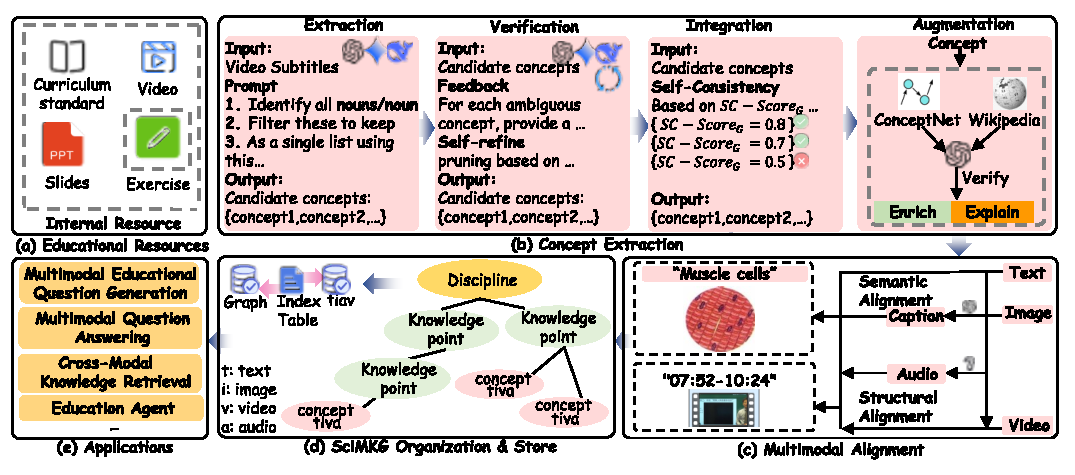
\includegraphics[width=\textwidth]{figures/fig_sm_overview_paper.pdf}
\caption{Khung xây dựng \SM{} (Hình 2 trong~\cite{lu2026scimkg}, giữ nguyên nhãn tiếng Anh của tác giả). \textbf{(a)} Tài nguyên giáo dục đầu vào: chuẩn chương trình, video, slide và bài tập. \textbf{(b)} Trích xuất khái niệm bằng chuỗi EVIA (Extraction, Verification, Integration, Augmentation). \textbf{(c)} Căn chỉnh đa phương thức: căn chỉnh ngữ nghĩa cho ảnh qua mô tả, căn chỉnh cấu trúc cho video và âm thanh. \textbf{(d)} Tổ chức và lưu trữ theo ba tầng môn học, điểm kiến thức và khái niệm. \textbf{(e)} Các ứng dụng của đồ thị.}
\label{fig:sm-pipeline}
\end{figure*}

\subsection{Thu thập và tiền xử lý}\label{sec:sm-preprocess}
Dữ liệu nguồn là video, slide và bài tập của các khóa học trực tuyến mở, kèm chuẩn chương trình.
Phụ đề của video được trích thành văn bản để tìm khái niệm, còn ảnh được tách từ slide để bổ sung phương thức cho khái niệm.
Để lời giảng rõ ràng và dễ tiếp cận hơn, bài báo dùng MLLM viết lại văn bản đã trích, sinh âm thanh tương ứng và ghi lại URL của từng video gốc.
Theo mã nguồn, văn bản là kết quả nhận dạng giọng nói (bước này làm thủ công, nằm ngoài mã; xem Mục~\ref{sec:sm-mismatch}).
Gemini gộp văn bản đó theo ngữ nghĩa thành các đoạn có mốc thời gian, và video được cắt thành các clip theo mốc đó.
Toàn bộ văn bản là tiếng Trung giản thể.

\subsection{Trích xuất khái niệm: chuỗi EVIA}\label{sec:sm-evia}
Chuỗi EVIA đã nêu ở phần tổng quan chạy trên từng đoạn phụ đề theo bốn bước.
Đầu vào của bước trích xuất (E) là văn bản của một đoạn; LLM xác định mọi danh từ và cụm danh từ rồi giữ lại những cụm thuộc môn học, và đầu ra là tập khái niệm ứng viên của đoạn.
Chẳng hạn, từ một đoạn nói về mô biểu bì, ứng viên có thể gồm ``mô biểu bì'', ``tế bào cơ'', ``hệ thống'', ``kính hiển vi'' và ``cơ quan'' (ví dụ minh họa của nhóm, không phải dữ liệu của bài).

Bước kiểm chứng (V) nhận tập ứng viên đó và trả về chính tập ấy kèm một điểm phiếu cho từng ứng viên.
Mỗi LLM trong ba LLM chạy năm vòng Self-Refine~\cite{madaan2023selfrefine}.
Ở mỗi vòng, LLM tự kiểm tra từng ứng viên có thuộc môn học hay không và nêu lý do ngắn cho ứng viên có thể bị loại (phản hồi), rồi lọc lại danh sách dựa trên các phản hồi đã tích lũy (sửa).
Ứng viên còn lại sau bước sửa được cộng một phiếu, nên điểm tối đa là 15.

Bước tích hợp (I) gộp các phiếu theo tinh thần Self-Consistency~\cite{wang2023selfconsistency}: ứng viên được nhiều mô hình và nhiều vòng giữ lại thì đáng tin hơn.
Ứng viên được giữ khi điểm tổng hợp đạt ngưỡng $\alpha=0{,}7$, mà bài mô tả là tần suất ứng viên được nhận ở bước kiểm chứng; nhóm hiểu đó là tỉ lệ phiếu trên số phiếu tối đa, tức ít nhất 11 trên 15 phiếu.
Trong ví dụ, ``mô biểu bì'' (15 phiếu), ``tế bào cơ'' (14) và ``cơ quan'' (11) được giữ, còn ``hệ thống'' và ``kính hiển vi'' (3 phiếu) bị loại.
Theo bài, Self-Refine làm sạch danh sách nên precision tăng, còn dùng nhiều LLM giúp không bỏ sót nên recall tăng; Mục~\ref{sec:sm-exp-pub} đối chiếu cách giải thích này với số liệu ablation, và Mục~\ref{sec:sm-ex02} kiểm tra lại tác động của kiểm chứng trên nhãn công bố.

Bước bổ sung (A) nhận tập khái niệm của I và trả về tập mở rộng cùng lời giải thích cho từng khái niệm, vì phụ đề chỉ chứa những gì giáo viên nói ra.
Mỗi khái niệm được tra trên ConceptNet để lấy các khái niệm lân cận theo tám quan hệ (IsA, RelatedTo, HasContext, PartOf, DefinedAs, Synonym, DerivedFrom, HasPrerequisite), qua các luật biểu thức chính quy do tác giả thiết kế; LLM sau đó lọc và kiểm tra chéo để chỉ giữ khái niệm thuộc môn học.
Các khái niệm này được liên kết với Wikipedia để lấy mô tả chi tiết, và LLM tóm tắt thành một câu giải thích ngắn gọn; bài báo coi việc bám Wikipedia là cách giảm ảo giác.

\subsection{Căn chỉnh đa phương thức}\label{sec:sm-align}
Căn chỉnh gắn từng phương thức vào khái niệm đã trích, nhờ khả năng hiểu liên phương thức của các MLLM.
Với ảnh, một MLLM ánh xạ mỗi ảnh vào khái niệm tương ứng bằng cách sinh mô tả ngữ nghĩa, rồi một MLLM khác kiểm tra cặp đó bằng cách chấm độ tin cậy dựa trên văn bản; chỉ những cặp có độ tin cậy trên 0,8 được giữ.
Với video, mỗi đoạn video được gắn với các khái niệm cùng xuất hiện trong đoạn đó, dựa trên ngữ nghĩa của văn bản khái niệm kết hợp với cấu trúc thời gian từ mốc thời gian, kèm URL để truy cập video gốc.
Với âm thanh, lời giải thích của khái niệm được viết lại dựa trên tri thức Wikipedia để giảm ảo giác, rồi chuyển thành âm thanh bằng TTS.

\subsection{Tổ chức và lưu trữ}\label{sec:sm-store}
\SM{} có ba tầng: tầng môn học ở trên cùng gồm sinh học, vật lý và hóa học; tầng điểm kiến thức ở giữa, tổ chức theo chuẩn chương trình và đề cương của các khóa MOOC; tầng khái niệm ở dưới cùng, chứa mọi khái niệm đa phương thức.
Môn học, điểm kiến thức, bài tập và khái niệm đa phương thức đều có mã định danh riêng và được liên kết thành một đồ thị phân cấp qua cơ chế tham chiếu chéo, lưu trong các bảng tham chiếu dạng JSON; đồ thị còn được xuất sang RDF tuân thủ IRI để dễ tái sử dụng.

Mỗi khái niệm và mỗi dữ liệu đa phương thức là một thực thể riêng, nối với nhau bằng mười một loại quan hệ: giải thích, ảnh, video và âm thanh (mỗi loại có một cặp quan hệ thuận và nghịch với khái niệm), quan hệ ``related to'' nối khái niệm với điểm kiến thức, và cặp quan hệ nối bài tập với điểm kiến thức.
Tổng cộng đồ thị có 1.356 điểm kiến thức, 34.630 khái niệm, 403.400 bộ ba, 763 bài tập, 10.527 ảnh, 10.425 video và 34.630 tệp âm thanh; ảnh phủ 39\% khái niệm, video phủ 80\% và âm thanh phủ 100\%.

\subsection{Bổ sung từ mã nguồn và điểm không khớp với bài báo}\label{sec:sm-mismatch}
Bài báo chỉ mô tả ở mức khái quát, nên nhóm đối chiếu với mã công bố~\cite{kgbnu2026scimkgcode}.
Các điểm đáng chú ý:
\begin{itemize}
\item \textbf{Tiền xử lý.} Nhận dạng giọng nói làm thủ công, ngoài mã; việc gộp đoạn bằng Gemini, cắt clip và tách ảnh nằm ở các hàm và dịch vụ ngoài rời nhau, phần điều phối chỉ còn ở dạng dòng chú thích. Phát biểu cuối của mỗi tài liệu bị bỏ.
\item \textbf{Trích xuất (E).} Chỉ gọi DeepSeek-V3, không phải nhiều LLM như bài mô tả. Một danh sách khái niệm đã gặp dùng chung cho toàn bộ dữ liệu, nên khái niệm chỉ gắn với lần giảng đầu tiên (mốc thời gian và clip).
\item \textbf{Kiểm chứng (V).} Prompt nhắm vào thuật ngữ mơ hồ liên ngành và dụng cụ thí nghiệm; mỗi vòng sửa luôn xuất phát từ danh sách ban đầu, nên giống lấy mẫu lặp hơn là sửa dần.
\item \textbf{Tích hợp (I).} Hệ số chuẩn hóa bằng 1 và điểm khởi tạo là 1, nên điều kiện ngưỡng 0,7 luôn đúng và, theo cách nhóm đọc mã, mọi ứng viên đều được giữ. Đây là nhận xét về mã công bố, không phải về cách dữ liệu công bố được sinh ra.
\item \textbf{Bổ sung (A).} Bộ luật cho ConceptNet để trống; khái niệm được dịch bằng Baidu Translate để tra Wikipedia; nhánh ``không tìm thấy trang'' không bao giờ chạy vì lỗi kiểu dữ liệu.
\item \textbf{Căn chỉnh.} Ảnh: GPT-4o gọi ba lần rồi lấy hợp, không có MLLM thứ hai và ngưỡng 0,8; ảnh còn bổ sung khái niệm mới. Video: mã trong repo chỉ cắt clip; bước dựng bộ ba có đọc trường URL video của từng khái niệm, nhưng không có mã nào tạo trường này. Gói \texttt{scimkg} 0.1.1 trên TestPyPI có ghép khái niệm với clip theo mốc thời gian, nhưng chỉ trả kết quả cho trang web minh họa, không đưa vào bộ ba hay RDF. Âm thanh: mô hình tts-1 của OpenAI.
\item \textbf{Lưu trữ.} Mỗi khái niệm sinh ít nhất 6 bộ ba theo cặp thuận-nghịch, thêm 2 cho mỗi liên kết khái niệm-ảnh và 2 cho mỗi liên kết khái niệm-video, nên tổng hơn 400 nghìn bộ ba; số liên kết lớn hơn số ảnh (10.527) vì một ảnh có thể gắn với nhiều khái niệm; ánh xạ RDF của video dùng khóa ``an video'', khác nhãn ``a video'' lúc sinh bộ ba.
\end{itemize}

% ------------------------------------------------------------
\section{Thực nghiệm}\label{sec:sm-exp}
% ------------------------------------------------------------
Bài báo đo chất lượng trích xuất và căn chỉnh nhưng không nêu chi phí chạy: toàn văn không có số token, giá hay tiền nào.
Với một đồ thị phủ hơn một nghìn điểm kiến thức, đây lại là điều người muốn áp dụng cần biết trước.
Phần này trả lời ba câu hỏi: (1) dựng một bài học tốn bao nhiêu lời gọi và token; (2) kiểm chứng đổi được bao nhiêu chất lượng với chi phí thêm bao nhiêu; (3) chỉ mục theo khái niệm của đồ thị tìm đúng đoạn bài giảng tốt đến đâu so với mốc ngẫu nhiên và mốc chỉ dùng văn bản.
Với câu (1), nhóm đo bằng số lượt gọi và số token, vì tiền phụ thuộc mô hình và bảng giá thay đổi theo thời điểm; tiền chỉ được quy đổi cho gpt-6-luna, mô hình đã dùng.
Ex01 (Mục~\ref{sec:sm-ex01}) trả lời câu (1) cho một bài học.
Ex02 (Mục~\ref{sec:sm-ex02}) đổi số vòng kiểm chứng để trả lời câu (2).
Ex03 (Mục~\ref{sec:sm-ex03}) trả lời câu (3) trên cùng sáu bài.
Trừ Mục~\ref{sec:sm-exp-pub}, mọi số đo ở đây đến từ bộ chạy của nhóm (Mục~\ref{sec:sm-exp-setup}).

\subsection{Kết quả công bố làm mốc tham chiếu}\label{sec:sm-exp-pub}
Bảng~\ref{tab:sm-pub} lấy lại kết quả trích xuất khái niệm của bài trên tập đánh giá gồm 100 bài học và 4.479 khái niệm; các baseline dựa trên LLM đều dùng GPT-4o.
Phương pháp đầy đủ đạt F1 cao nhất, 0,803.
Các dòng ``EVIA w/o \dots'' là phần cắt bỏ: ``MLs'' là nhiều LLM, còn ``SF-FD'' là vòng tự phản hồi.
Bài còn quét số vòng lặp và ngưỡng trên chín tổ hợp; cấu hình 5 vòng, ngưỡng 0,7 cho F1 tốt nhất.
Về căn chỉnh ảnh, bài nêu bốn điểm tự động (CLIP 0,83, BLIP-ITM 0,76, X-VLM-ITM 0,81, VQAScore 0,75) và điểm trung bình 0,73 của năm chuyên gia; căn chỉnh video và âm thanh không được đo.

\begin{table}[t]
\centering
\caption{Trích xuất khái niệm theo bài báo (chọn lọc).}
\label{tab:sm-pub}
\small
\setlength{\tabcolsep}{4pt}
\resizebox{\columnwidth}{!}{%
\begin{tabular}{@{}lcccc@{}}
\toprule
Phương pháp & P & R & F1 & MCC \\
\midrule
Decomposed-QA & 0,935 & 0,570 & 0,712 & \textbf{0,741} \\
GPT-NER & 0,530 & \textbf{0,931} & 0,681 & 0,621 \\
LinkNER & 0,855 & 0,644 & 0,734 & 0,732 \\
UniversalNER & 0,873 & 0,617 & 0,718 & 0,722 \\
\midrule
EVIA, Qwen3-14B+Gemma3-27B+Phi-3-14B & 0,879 & 0,637 & 0,739 & 0,730 \\
EVIA w/o MLs$^{a}$ & 0,769 & 0,342 & 0,477 & 0,509 \\
EVIA w/o SF-FD & 0,374 & 0,589 & 0,459 & 0,428 \\
EVIA w/o MLs + SF-FD$^{b}$ & 0,340 & 0,290 & 0,312 & 0,315 \\
\textbf{EVIA (đầy đủ)} & \textbf{0,947} & 0,702 & \textbf{0,803} & 0,729 \\
\bottomrule
\end{tabular}}
\par\smallskip
{\footnotesize\raggedright $^{a}$Một mô hình, có vòng tự phản hồi: gần cấu hình đầy đủ của Ex02. $^{b}$Một mô hình, dùng thẳng kết quả trích xuất: gần cấu hình tắt kiểm chứng của Ex02.\par}
\end{table}

Nhóm dùng các số này làm mốc về hướng, không làm mốc về giá trị.
Bài chạy nhiều LLM thương mại trên 100 bài, còn Ex02 chạy một mô hình trên sáu bài.
Theo hai dòng này, vòng tự phản hồi nâng F1 từ 0,312 lên 0,477, chủ yếu nhờ precision (từ 0,340 lên 0,769).
Hai dòng ``EVIA w/o MLs'' và ``EVIA (đầy đủ)'' cho thấy dùng nhiều LLM nâng recall từ 0,342 lên 0,702, đúng như bài giải thích, nhưng precision cũng tăng từ 0,769 lên 0,947; vậy nhiều LLM không chỉ giúp bớt bỏ sót mà còn lọc bớt ứng viên sai.

\subsection{Thiết lập thực nghiệm}\label{sec:sm-exp-setup}
\textbf{Dữ liệu.}
Nhóm lấy sáu bài từ bộ MOOC mà tác giả công bố, mỗi môn (sinh học, vật lý, hóa học) hai bài (Bảng~\ref{tab:sm-lessons}); bộ này kèm tập nhãn khái niệm chuẩn (ground truth) theo từng bài, và nhóm dùng tập nhãn đó để chấm.
Văn bản đưa vào mô hình và nhãn dùng để chấm được tách riêng; nhãn không được đọc hay gửi đi trong quy trình dựng đồ thị.
Văn bản bài giảng bằng tiếng Trung được giữ nguyên, chỉ tên bài ghi bằng tiếng Việt.
Bộ công bố có văn bản và ảnh nhưng không có video và PDF gốc, nên ba thực nghiệm này không dùng video.
Ex01 dùng 27 ảnh slide của bài Cấu tạo hệ thần kinh; Ex02 và Ex03 chỉ dùng văn bản.

\begin{table}[t]
\centering
\caption{Sáu bài dùng trong thực nghiệm (bộ MOOC do tác giả công bố).}
\label{tab:sm-lessons}
\small
\begin{tabular}{@{}llrr@{}}
\toprule
Bài & Môn & Đoạn & Nhãn \\
\midrule
Cấu tạo hệ thần kinh & Sinh học & 14 & 30 \\
Sinh sản của động vật lưỡng cư & Sinh học & 7 & 57 \\
Áp suất khí quyển & Vật lý & 12 & 21 \\
Lực đẩy & Vật lý & 14 & 19 \\
Axit sunfuric và muối sunfat & Hóa học & 15 & 13 \\
Protein & Hóa học & 13 & 48 \\
\midrule
\textbf{Tổng} & & \textbf{75} & \textbf{188} \\
\bottomrule
\end{tabular}
\end{table}

\textbf{Cấu hình và khác biệt so với bài.}
Trong cả ba thực nghiệm, mọi lời gọi LLM dùng một mô hình duy nhất là gpt-6-luna ở mức suy luận thấp, gọi qua công cụ dòng lệnh bằng tài khoản thuê bao, thay cho nhiều LLM của bài.
Nhóm giữ số vòng kiểm chứng bằng 5 và ngưỡng 0,7 như bài.
Điều kiện tích hợp trong mã công bố được nhóm đọc là luôn đúng, nên mọi ứng viên đều được giữ (Mục~\ref{sec:sm-mismatch}).
Bộ chạy của nhóm sửa điều này: điểm tích hợp là số phiếu của kiểm chứng chia cho số phiếu tối đa (số mô hình nhân số vòng), và ngưỡng 0,7 có tác dụng thật.
Với một mô hình, năm vòng cần ít nhất bốn phiếu (4 trên 5 là 0,8, đạt ngưỡng; 3 trên 5 là 0,6, không đạt), còn một vòng cần đúng một phiếu.
Các khác biệt còn lại: căn chỉnh ảnh không có ngưỡng 0,8 của bài báo; lời giải thích tra Wikipedia tiếng Trung bằng đúng tên khái niệm và lấy các đoạn văn dài từ 30 ký tự, thay cho bước dịch bằng Baidu Translate rồi tra Wikipedia của mã gốc, vì bước đó cần khóa dịch vụ và máy chủ trung gian (Mục~\ref{sec:sm-mismatch});tiền xử lý dùng văn bản và ảnh đã công bố thay cho bước thủ công của mã gốc; tập khái niệm đã gặp được đặt lại theo từng bài.
Bộ luật dựa trên sáu mẫu câu tiếng Anh của ConceptNet, bỏ Synonym và DerivedFrom, và khớp mọi thuật ngữ đã tra thay vì chỉ thuật ngữ cuối như mã gốc.
Vì API ConceptNet trả lỗi 502 khi chạy, truy vấn được trả lời từ bản dump 5.7.0 đã công bố, đọc thành cùng cấu trúc dữ liệu mà mã gốc đọc từ API.

\subsection{Ex01: chi phí một bài học}\label{sec:sm-ex01}
Ex01 chạy trọn bài ``Cấu tạo hệ thần kinh'' (14 đoạn, 27 ảnh) từ văn bản đến đồ thị bằng một luồng duy nhất; Bảng~\ref{tab:sm-ex01-cost} tách số đo theo từng bước.

\textbf{Cách đo chi phí.}
Các lượt chạy dùng tài khoản thuê bao nên không có hóa đơn theo token.
Vì vậy nhóm đếm token theo hai cách và dùng hai số đó để ước lượng tiền, một số cao và một số thấp.
Cách thứ nhất lấy số do công cụ dòng lệnh báo, gọi là token CLI.
Số này lớn, nhiều khả năng vì công cụ gửi kèm một phần nội dung cố định của nó trong mỗi lượt (xem nhận xét 3 bên dưới).
Công cụ cũng cho biết bao nhiêu token đầu vào là phần lặp lại của lượt trước; nhà cung cấp giữ sẵn phần này (cached input) nên tính giá rẻ hơn.
Cách thứ hai chỉ đếm nội dung do nhóm soạn: prompt, schema và ảnh, gọi là token kiểu API.
Chữ được đếm bằng bộ tách từ \texttt{o200k\_base}, còn ảnh được ước lượng theo quy tắc tính token ảnh của OpenAI.
Số này nhỏ hơn token CLI vì không có phần nội dung cố định.
Cách này không biết phần nào được lưu sẵn, nên nhóm tính mọi token vào theo giá thường.
Số lượt gọi và số token ra giống nhau ở cả hai cách.
Token CLI cho số tiền cao (cận trên), token kiểu API cho số tiền thấp (cận dưới).
Ex01 có cả hai (Bảng~\ref{tab:sm-ex01-cost}); Ex02 chỉ in token kiểu API nên chỉ có cận dưới.
Mọi lượt gọi trong Ex01 và Ex02 đều có số token; lượt nào dùng lại kết quả đã lưu cục bộ thì không gửi yêu cầu mới và không được tính thêm.


Quy ra tiền dùng giá nhập, giá nhập đã lưu sẵn và giá xuất của mô hình, tính cho một triệu token: token vào chưa lưu sẵn nhân giá nhập, cộng token vào đã lưu sẵn nhân giá nhập đã lưu sẵn, cộng token ra nhân giá xuất.
Với gpt-6-luna (giá nhập 0,10 USD, giá nhập đã lưu sẵn 0,01 USD, giá xuất 0,50 USD), cận dưới 0,027 USD dùng token kiểu API và coi mọi token vào là chưa lưu sẵn; cận trên 0,19 USD dùng token CLI.
Hai cận này chưa thật chặt.
Nếu một phần đầu vào được lưu sẵn, chi phí thấp hơn cận dưới tối đa khoảng 0,018 USD.
Cận trên không tính phụ phí ghi vào bộ nhớ đệm, vì công cụ dòng lệnh không báo số token ghi; nếu tính mọi token vào chưa lưu sẵn theo giá ghi 0,125 USD mỗi triệu token, cận trên lên khoảng 0,23 USD.

% Bảng sinh tự động từ số đo bằng report/tools/make_ex_tables.py; không sửa tay.
\begin{table*}[t]
\centering
\caption{Chi phí Ex01 theo bước, lượt gpt-6-luna trên bài ``Cấu tạo hệ thần kinh''. Token vào CLI gồm ngữ cảnh cố định của công cụ; token vào kiểu API là số đếm trên prompt và schema, cộng token ảnh ước lượng. Chưa gồm tiền xử lý và ghép, cắt video (không đo được vì thiếu video và PDF gốc); tạo âm thanh chạy cục bộ nên không có lượt gọi.}
\label{tab:sm-ex01-cost}
\small
\setlength{\tabcolsep}{3pt}
% Generated by report/tools/make_ex_tables.py from measured run files; do not edit by hand.
\begin{tabular}{@{}lrrrrrrr@{}}
\toprule
Bước & Lượt gọi & \begin{tabular}[c]{@{}r@{}}Token vào,\\CLI\end{tabular} & \begin{tabular}[c]{@{}r@{}}trong đó\\đã lưu sẵn\end{tabular} & \begin{tabular}[c]{@{}r@{}}Token vào,\\kiểu API\end{tabular} & Token ra & \begin{tabular}[c]{@{}r@{}}Tỉ lệ\\tổng token\end{tabular} & Thời gian (phút) \\
\midrule
Trích xuất (E) & 14 & 176.344 & 48.128 & 3.532 & 676 & 4,1\% & 1,2 \\
Kiểm chứng (V) & 120 & 1.525.309 & 986.624 & 43.995 & 6.298 & 35,3\% & 10,3 \\
Tích hợp (I) & 0 & 0 & 0 & 0 & 0 & 0,0\% & 0,0 \\
Bổ sung (A) và truy hồi nguồn & 16 & 201.026 & 84.224 & 3.548 & 699 & 4,6\% & 1,3 \\
Tạo giải thích & 104 & 1.351.503 & 950.528 & 67.559 & 4.224 & 31,2\% & 10,7 \\
Căn chỉnh ảnh & 81 & 1.071.750 & 709.888 & 76.215 & 3.012 & 24,8\% & 7,7 \\
Tạo âm thanh (cục bộ) & 0 & 0 & 0 & 0 & 0 & 0,0\% & 0,6 \\
\midrule
\textbf{Tổng} & \textbf{335} & \textbf{4.325.932} & \textbf{2.779.392} & \textbf{194.849} & \textbf{14.909} & \textbf{100\%} & \textbf{31,8} \\
\bottomrule
\end{tabular}

\end{table*}

Đầu ra gồm 38 khái niệm sau kiểm chứng và tích hợp; bước bổ sung từ ConceptNet thêm 64 khái niệm và căn chỉnh ảnh thêm 2, thành 104 khái niệm cuối.
Mỗi khái niệm cuối có một giải thích: 82 có văn bản Wikipedia tiếng Trung dùng được, còn 22 khái niệm không có trang trùng tên (lỗi 404) nên dùng giải thích dự phòng của mô hình và được gắn nhãn không có nguồn.
Văn bản nguồn của 23 giải thích chưa nằm trong Bảng~\ref{tab:sm-ex01-cost}; phần này làm tổng token vào chênh dưới 1\%.
Đồ thị gồm 744 bộ ba, tương ứng 1.097 câu lệnh RDF, kèm 104 tệp âm thanh (tổng khoảng 733 giây).

Bảng~\ref{tab:sm-ex01-cost} cho ba nhận xét.
\begin{enumerate}
\item Ba bước kiểm chứng, tạo giải thích và căn chỉnh ảnh chiếm khoảng 91\% token CLI. Kiểm chứng gọi mô hình 120 lần: mỗi vòng có hai lượt (phản hồi rồi sửa), năm vòng là 10 lượt cho một đoạn, và chỉ 12 trong 14 đoạn được kiểm chứng. Hai đoạn còn lại (đoạn 9 và 12) không còn ứng viên, vì mọi khái niệm trích được ở đó đã xuất hiện ở đoạn trước, mà mã chỉ giữ lần xuất hiện đầu tiên và bỏ qua kiểm chứng khi đoạn rỗng. Tích hợp và xuất đồ thị chạy bằng mã nên không có lượt gọi.
\item Bước bổ sung từ ConceptNet tốn ít token nhưng thêm 64 khái niệm, nhiều hơn số còn lại sau kiểm chứng. Đây là số khái niệm được thêm, chưa phải số khái niệm đúng: Ex02 chấm ngay sau bước tích hợp, trước khi bổ sung, và nhãn của tác giả chỉ gồm khái niệm có trong bài nên không chấm được phần bổ sung (không khái niệm nào trùng hẳn nhãn).
\item Mỗi lượt có khoảng 12.560 đến 13.230 token vào CLI, trong khi mỗi giải thích chỉ trả về khoảng 41 token ra. Ở các bước chỉ có chữ, token kiểu API chỉ chiếm khoảng 2 đến 5\% token CLI; ở bước căn chỉnh ảnh, token kiểu API (gồm cả token ảnh ước lượng) chiếm khoảng 7\%, trong đó phần chữ khoảng 4\%. Phần chênh là ngữ cảnh cố định mà công cụ tự thêm vào mỗi lượt: ở 254 lượt chỉ có chữ, token vào CLI trừ đi token của prompt và schema luôn nằm trong khoảng 12.339 đến 12.350, dù prompt dài từ 127 đến 3.457 token. Tính cho cả 335 lượt, phần cố định này khoảng 4,14 triệu token, tức khoảng 96\% token vào CLI.
\end{enumerate}

Đếm theo kiểu API, tổng token vào là 194.849, trong đó 30.855 là token ảnh ước lượng (mỗi ảnh được gửi ba lần) và 163.994 là văn bản; tổng này bằng khoảng 4,5\% token vào CLI.
Nếu phần cố định ở lượt có ảnh cũng như ở lượt chỉ có chữ, token ảnh suy từ số CLI là khoảng 26.400, thấp hơn ước lượng khoảng 14\%, nên số ước lượng hơi cao.
Hai cách đếm cho cận dưới và cận trên khác nhau khoảng 7 lần ở gpt-6-luna (0,027 so với 0,19 USD), nhỏ hơn nhiều so với tỉ lệ khoảng 22 lần giữa hai cách đếm token vào (194.849 so với 4.325.932 token).
Khoảng cách hẹp lại vì hai lý do: khoảng 64\% token vào CLI được tính theo giá đã lưu sẵn, rẻ hơn giá bình thường, trong khi token vào kiểu API bị coi là chưa lưu sẵn toàn bộ; và token ra, giống nhau ở cả hai cách, chiếm một phần chi phí không đổi theo cách đếm token vào, nên kéo tỉ lệ chi phí lại gần hơn tỉ lệ token.
Báo cáo ghi cả hai cận thay vì chọn một.
Cận trên cao hơn thực tế vì gồm phần ngữ cảnh cố định của công cụ nói trên; cận dưới có thể thấp hơn thực tế, vì một chương trình gọi API thật có thể gửi thêm nội dung mà đếm này không có.
Tiền xử lý và ghép, cắt video không đo được vì nhóm không có video và PDF gốc của bài; các bước này có thể làm chi phí thực tế cao hơn.
\wandb{https://wandb.ai/nhinbm-hcmus/SciMKG/runs/7b20992d11ea}

\subsection{Ex02: kiểm chứng đổi được gì}\label{sec:sm-ex02}
Ex02 đo kiểm chứng (V) đổi được bao nhiêu chất lượng khái niệm.
Nhóm chọn V vì đây là bước tốn nhiều lời gọi và token CLI nhất ở Ex01: 120 trong 335 lượt gọi và 35,3\% tổng token CLI (Bảng~\ref{tab:sm-ex01-cost}).

\textbf{Thiết kế.}
Nhóm chỉ đổi số vòng kiểm chứng: 0 vòng, 1 vòng, và 5 vòng như bài báo; ở 0 vòng V không được gọi nên tập chấm chính là ứng viên của E.
Mô hình, tham số và cách dựng đầu vào giữ như Ex01.
Mỗi cấu hình chạy các bước E, V, I và A trên văn bản của sáu bài, không chạy ảnh và giải thích, nên chi phí chỉ gồm các bước này.
E được gọi lại ở mỗi cấu hình, nên ba cấu hình có ba lượt E khác nhau trên cùng đầu vào; riêng bài Cấu tạo hệ thần kinh ở 5 vòng dùng lại kết quả của Ex01.

\textbf{Cách chấm.}
Nhóm chấm ngay sau bước tích hợp (I), trên nhãn công bố: với mỗi bài, gộp khái niệm của mọi đoạn, loại trùng, rồi so với nhãn của đúng bài đó.
Bước bổ sung (A) không được chấm, vì phép chấm đặt trước A và nhãn chỉ gồm khái niệm có trong bài (nhận xét 2 ở Mục~\ref{sec:sm-ex01}).
Bỏ A không đổi precision, recall hay F1 nên nhóm không lập cấu hình tắt bổ sung; A vẫn chạy để Ex03 (Mục~\ref{sec:sm-ex03}) dùng lại ba đồ thị đầy đủ.
Nếu chấm cả phần bổ sung, recall chỉ tăng 0,005 đến 0,011 (mỗi cấu hình chỉ khớp thêm hai nhãn trên sáu bài), còn precision giảm từ khoảng 0,30--0,34 xuống 0,07--0,09 và F1 giảm khoảng 0,23 đến 0,26.
Vì nhãn chỉ gồm khái niệm có trong bài, số này cho thấy A chủ yếu thêm khái niệm ngoài bài, chưa cho biết chúng đúng hay sai.
Chỉ số chính là khớp đúng từng chuỗi sau chuẩn hóa NFKC và đổi phồn thể sang giản thể bằng OpenCC, cùng phép chuẩn hóa mà đường ống dùng để loại trùng ở bước gộp.
Khớp chuỗi con (một bên chứa bên kia, chuỗi ngắn có ít nhất hai ký tự) chỉ dùng để thăm dò.
Precision tính trên khái niệm dự đoán, recall tính trên nhãn; nhóm tính từng bài rồi lấy trung bình cộng sáu bài.
Mỗi lượt cũng ghi trần recall của E, tức recall của toàn bộ ứng viên trước khi V lọc.
Nhãn công bố có thể thiếu khái niệm đúng, và một dự đoán đúng nhưng không có trong nhãn vẫn bị tính sai; vì vậy precision đo được là cận dưới của precision thật, còn recall chỉ đo độ phủ trên nhãn đã có.

\begin{table}[t]
\centering
\caption{Ex02: trung bình sáu bài theo số vòng kiểm chứng. F1 là trung bình của F1 từng bài nên không bằng trung bình điều hòa của hai dòng đầu. Chi phí tính theo giá gpt-6-luna, chỉ cho E, V và A trên văn bản (không gồm ảnh và giải thích).}
\label{tab:sm-ex02-summary}
\footnotesize
\resizebox{\columnwidth}{!}{% Generated by report/tools/make_ex_tables.py from measured run files; do not edit by hand.
\begin{tabular}{@{}lccc@{}}
\toprule
Chỉ số (trung bình sáu bài) & 0 vòng & 1 vòng & 5 vòng \\
\midrule
Precision & 0,302 & 0,327 & 0,344 \\
Recall & 0,634 & 0,455 & 0,450 \\
F1 & 0,392 & 0,362 & 0,373 \\
F1 khớp chuỗi con (thăm dò) & 0,560 & 0,543 & 0,539 \\
Trần recall của E & 0,634 & 0,627 & 0,609 \\
Số lời gọi, sáu bài & 254 & 335 & 882 \\
Token vào, kiểu API & 73.829 & 102.910 & 330.238 \\
Token ra, kiểu API & 14.641 & 21.868 & 54.166 \\
Chi phí, USD (Luna, cận dưới) & 0,015 & 0,021 & 0,060 \\
Bài có F1 thấp hơn cấu hình 5 vòng & 2 / 6 & 4 / 6 & – \\
\bottomrule
\end{tabular}
}
\end{table}

\begin{table*}[t]
\centering
\caption{Ex02: precision (P), recall (R) và F1 từng bài theo số vòng kiểm chứng, khớp đúng sau chuẩn hóa. Mỗi ô là một lần chạy.}
\label{tab:sm-ex02-quality}
\footnotesize
\setlength{\tabcolsep}{4pt}
% Generated by report/tools/make_ex_tables.py from measured run files; do not edit by hand.
\begin{tabular}{@{}lccccccccc@{}}
\toprule
 & \multicolumn{3}{c}{0 vòng} & \multicolumn{3}{c}{1 vòng} & \multicolumn{3}{c}{5 vòng (đầy đủ)} \\
\cmidrule(lr){2-4}\cmidrule(lr){5-7}\cmidrule(l){8-10}
Bài & P & R & F1 & P & R & F1 & P & R & F1 \\
\midrule
Cấu tạo hệ thần kinh & 0,435 & 0,900 & 0,587 & 0,468 & 0,733 & 0,571 & 0,526 & 0,667 & 0,588 \\
Sinh sản của động vật lưỡng cư & 0,657 & 0,842 & 0,739 & 0,689 & 0,737 & 0,712 & 0,667 & 0,667 & 0,667 \\
Áp suất khí quyển & 0,167 & 0,333 & 0,222 & 0,286 & 0,191 & 0,229 & 0,250 & 0,191 & 0,216 \\
Lực đẩy & 0,118 & 0,316 & 0,171 & 0,067 & 0,105 & 0,082 & 0,120 & 0,158 & 0,136 \\
Axit sunfuric và muối sunfat & 0,132 & 0,769 & 0,225 & 0,107 & 0,462 & 0,174 & 0,132 & 0,538 & 0,212 \\
Protein & 0,301 & 0,646 & 0,411 & 0,343 & 0,500 & 0,407 & 0,371 & 0,479 & 0,418 \\
\midrule
\textbf{Trung bình} & \textbf{0,302} & \textbf{0,634} & \textbf{0,392} & \textbf{0,327} & \textbf{0,455} & \textbf{0,362} & \textbf{0,344} & \textbf{0,450} & \textbf{0,373} \\
\bottomrule
\end{tabular}

\end{table*}

Bảng~\ref{tab:sm-ex02-summary} và Bảng~\ref{tab:sm-ex02-quality} cho bốn nhận xét.
\begin{enumerate}
\item F1 thay đổi ít giữa ba cấu hình: 0,392 với 0 vòng, 0,362 với 1 vòng và 0,373 với 5 vòng. Trần recall của E dao động từ 0,609 đến 0,634 dù đầu vào giống nhau, vì E được gọi lại ở mỗi cấu hình; nhóm lấy mức 0,025 này làm ước lượng thô về độ nhiễu của một lần chạy. Chênh lệch F1 lớn nhất giữa các cấu hình (0,030) cùng cỡ mức đó, và mỗi ô chỉ có một lần chạy, nên nhóm chưa thể nói cấu hình nào tốt hơn.
\item Kiểm chứng làm recall giảm rõ nhưng chỉ nâng precision ít. Từ 0 vòng sang 5 vòng, recall giảm 0,184 (từ 0,634 xuống 0,450), lớn hơn nhiều mức nhiễu 0,025; precision tăng 0,042 (từ 0,302 lên 0,344), chỉ cùng cỡ mức nhiễu. Phần lớn thay đổi xảy ra ngay ở vòng đầu: từ 0 sang 1 vòng, recall giảm 0,179 và precision tăng 0,025; từ 1 sang 5 vòng, recall chỉ giảm thêm 0,005 và precision tăng thêm 0,017.
\item So với bài báo, precision đổi cùng chiều nhưng mức chênh khác nhiều, còn recall đổi ngược chiều. Trên một mô hình, bài báo cho thấy vòng tự phản hồi nâng precision từ 0,340 lên 0,769 và recall từ 0,290 lên 0,342 (Bảng~\ref{tab:sm-pub}, các dòng ``EVIA w/o MLs'' và ``EVIA w/o MLs + SF-FD''). Một giả thuyết là cấu hình 0 vòng của nhóm không lọc khái niệm nào, nên recall nền (0,634) cao hơn nhiều so với dòng tương ứng của bài; bài không mô tả đủ cách tạo dòng cắt bỏ này để kiểm tra giả thuyết đó.
\item Chất lượng không tăng theo chi phí. Năm vòng dùng 882 lời gọi, gấp 3,5 lần cấu hình 0 vòng (254 lời gọi), và chi phí kiểu API gấp khoảng bốn lần (0,060 so với 0,015 USD, theo giá gpt-6-luna). Mức tăng đến từ V: 700 lời gọi ở 5 vòng, tức 10 lời gọi cho mỗi đoạn có ứng viên (70 trong 75 đoạn), trong khi số lời gọi của A giảm từ 179 xuống 107. Chi phí tăng nhanh hơn số lời gọi vì lời gọi của V mang theo danh sách ứng viên và phản hồi các vòng trước, nên token vào kiểu API trung bình mỗi lời gọi tăng từ 291 lên 374.
\end{enumerate}

Trên sáu bài này, chưa thấy kiểm chứng làm tăng F1 trong khi nó làm chi phí tăng khoảng bốn lần.
Điều này chưa đủ để bỏ V, vì bài báo dùng ba mô hình khác nhau cho V, còn nhóm chỉ dùng một mô hình, sáu bài và một lần chạy cho mỗi ô.
\wandb{https://wandb.ai/nhinbm-hcmus/SciMKG/runs/ex02-8319b815}

\subsection{Ex03: tìm đúng đoạn bài giảng}\label{sec:sm-ex03}
Bài báo nói đồ thị gắn khái niệm với đoạn video để phục vụ truy hồi, nhưng không đo tác vụ nào.
Ex03 kiểm tra trên cùng sáu bài: cho một câu, đồ thị có chỉ ra đúng đoạn bài giảng chứa câu đó không.
Vì Ex02 không chạy căn chỉnh ảnh hay video, tác vụ này chỉ kiểm tra phần văn bản của đồ thị, chưa kiểm tra phần đa phương thức mà bài báo mô tả cho truy hồi.
Hỏi đáp trắc nghiệm bị loại vì các bộ có sẵn chỉ có từ 1 đến 38 câu khớp từ khóa mỗi bài.

\textbf{Truy vấn và đáp án.}
Nhóm tách bản ghi của sáu bài theo dấu câu, giữ các câu có ít nhất 15 ký tự, được 309 câu.
Đáp án là đoạn chứa câu đó theo mốc thời gian có sẵn; không ai gán nhãn.
Mỗi câu có hai dạng: câu nguyên văn, và câu viết lại thành câu hỏi kiểu học sinh, giữ thuật ngữ khoa học.
gpt-6-luna viết lại mỗi câu bằng một lời gọi (309 lời gọi), rồi cố định thành tập dùng chung cho mọi cách tìm.
Có 191 câu viết lại trên 50\% cặp ký tự trùng với câu gốc, nên bộ này có thể dễ hơn câu hỏi thật; chất lượng câu viết lại chưa được chấm.

\textbf{Cách tìm.}
Đồ thị gồm hai phần dùng ở đây: nút khái niệm và liên kết từ khái niệm tới đoạn.
Trước hết, mỗi đoạn được gắn các khái niệm của nó theo một trong hai cách.
Cách ``đoạn đầu'' chỉ gắn khái niệm vào đoạn đầu tiên trích ra nó, như mã công bố (Mục~\ref{sec:sm-mismatch}).
Cách ``mọi đoạn có nhắc'' gắn vào mọi đoạn có văn bản chứa khái niệm đó.
Khái niệm ConceptNet thêm vào được gắn cùng đoạn với khái niệm gốc sinh ra nó; khái niệm một ký tự bị bỏ.
Mỗi truy vấn cộng điểm cho từng khái niệm xuất hiện trong đó, sau khi chuẩn hóa chữ như Ex02; khái niệm càng ít đoạn chứa thì điểm càng cao (trọng số IDF).
Các đoạn được xếp theo điểm, và các đoạn bằng điểm được lấy trung bình trên mọi thứ tự có thể, nên kết quả không phụ thuộc may rủi.
Mỗi cấu hình Ex02 cho một danh sách khái niệm riêng, nên ba cấu hình được so trên cùng tác vụ.
Hai mốc không dùng khái niệm: ngẫu nhiên (mốc dưới), và BM25 trên toàn văn bản ghi, tách từ theo cặp hai chữ vì tiếng Trung không có dấu cách (mốc trên).
Hit@1 là tỉ lệ truy vấn có đoạn đúng đứng đầu, Hit@3 là tỉ lệ có đoạn đúng trong ba đoạn đầu, và MRR là trung bình của 1 chia cho thứ hạng đoạn đúng.
Độ phủ là tỉ lệ truy vấn chạm ít nhất một khái niệm; truy vấn không chạm khái niệm nào chỉ ngang chọn ngẫu nhiên.

\begin{table*}[t]
\centering
\caption{Ex03: tìm đúng đoạn bài giảng, trung bình sáu bài (309 truy vấn mỗi loại). Mốc dưới là ngẫu nhiên, mốc trên là BM25 trên toàn văn bản ghi.}
\label{tab:sm-ex03}
\footnotesize
\setlength{\tabcolsep}{3pt}
% Generated by report/tools/make_ex_tables.py from measured run files; do not edit by hand.
\begin{tabular}{@{}lrrrrrrrr@{}}
\toprule
 & \multicolumn{4}{c}{Câu nguyên văn} & \multicolumn{4}{c}{Câu viết lại} \\
\cmidrule(lr){2-5}\cmidrule(l){6-9}
Cách tìm & Hit@1 & Hit@3 & MRR & Độ phủ & Hit@1 & Hit@3 & MRR & Độ phủ \\
\midrule
Ngẫu nhiên (mốc dưới) & 0,085 & 0,256 & 0,260 & 0,000 & 0,085 & 0,256 & 0,260 & 0,000 \\
BM25 trên toàn văn bản ghi (mốc trên) & 1,000 & 1,000 & 1,000 & 1,000 & 0,900 & 0,970 & 0,936 & 1,000 \\
\midrule
Đồ thị, đoạn đầu, kiểm chứng 0 vòng & 0,483 & 0,717 & 0,626 & 0,910 & 0,290 & 0,544 & 0,466 & 0,789 \\
Đồ thị, đoạn đầu, kiểm chứng 1 vòng & 0,378 & 0,575 & 0,524 & 0,810 & 0,235 & 0,438 & 0,401 & 0,667 \\
Đồ thị, đoạn đầu, kiểm chứng 5 vòng & 0,376 & 0,588 & 0,528 & 0,771 & 0,224 & 0,426 & 0,392 & 0,581 \\
\midrule
Đồ thị, mọi đoạn có nhắc, kiểm chứng 0 vòng & 0,657 & 0,825 & 0,760 & 0,910 & 0,445 & 0,664 & 0,594 & 0,789 \\
Đồ thị, mọi đoạn có nhắc, kiểm chứng 1 vòng & 0,503 & 0,705 & 0,639 & 0,810 & 0,317 & 0,544 & 0,486 & 0,667 \\
Đồ thị, mọi đoạn có nhắc, kiểm chứng 5 vòng & 0,510 & 0,709 & 0,644 & 0,771 & 0,307 & 0,532 & 0,476 & 0,581 \\
\bottomrule
\end{tabular}

\end{table*}

Bảng~\ref{tab:sm-ex03} cho kết quả trung bình sáu bài, với ba điểm chính.
\begin{enumerate}
\item Gắn mọi đoạn có nhắc tốt hơn gắn đoạn đầu từ 8 đến 17 điểm Hit@1, vì cách của mã công bố bỏ lỡ nhiều đoạn có nhắc tới khái niệm.
\item Cấu hình 0 vòng tìm đúng đoạn tốt nhất ở cả hai loại truy vấn (Hit@1 là 0,657 và 0,445), dù precision thấp hơn. Điều này đi cùng độ phủ: 0,910 so với 0,771 của 5 vòng với câu nguyên văn, tức kiểm chứng làm nhiều câu không chạm khái niệm nào. Độ phủ chỉ giải thích một phần: khi chỉ xét các câu mà cả hai cấu hình đều chạm (226 câu nguyên văn, 169 câu viết lại) và gắn mọi đoạn có nhắc, 0 vòng vẫn cao hơn (0,732 so với 0,632; 0,592 so với 0,482). Với cách đoạn đầu, chênh lệch nhỏ hơn (0,520 so với 0,463) hoặc gần như không có (0,342 so với 0,339 với câu viết lại).
\item Với cách đoạn đầu, bước bổ sung (A) đổi Hit@1 không quá 0,004 ở mọi cấu hình và loại truy vấn, và tăng độ phủ từ 0,004 đến 0,034 (các dòng này không in trong bảng).
\end{enumerate}

Câu nguyên văn lấy từ chính văn bản dựng đồ thị, nên dễ hơn truy vấn thật; BM25 đạt 1,000 với loại này và là mốc trên, không phải đối thủ của đồ thị.
Một số câu chỉ là lời dẫn lớp học, nên câu viết lại từ đó mơ hồ với mọi cách tìm.
Đây là truy hồi chứ không phải hỏi đáp: nó đo đồ thị có tóm đúng nội dung từng đoạn không, chưa đo việc trả lời.
Mỗi cấu hình có một lần chạy.
\wandb{https://wandb.ai/nhinbm-hcmus/SciMKG/runs/krpbt4zl}

\subsection{Thảo luận và giới hạn}\label{sec:sm-exp-discuss}
\textbf{Giới hạn của số đo.}
Mọi số chi phí là của một mô hình ở mức suy luận thấp, và chỉ đo trên sáu bài (Ex01 chỉ một bài).
Trong 104 giải thích, 22 không có văn bản nguồn (Mục~\ref{sec:sm-ex01}); tỉ lệ này phản ánh cách tra của nhóm, không phải thiết kế của bài.

\textbf{Điểm cần thận trọng trong số liệu công bố.}
Bài nói phương pháp của họ đứng đầu ở F1, ACC và AUC, nhưng ở MCC thì không: 0,729, so với 0,741 của Decomposed-QA và 0,732 của LinkNER (Bảng~\ref{tab:sm-pub}).
Các chỉ số đo khác nhau nên thứ hạng có thể đổi: Decomposed-QA thấp hơn bài 0,091 ở F1 nhưng cao hơn 0,012 ở MCC.
MCC tính cả hai loại đúng và hai loại sai, có giá trị từ -1 đến 1; càng gần 1 càng tốt.
ACC là tỉ lệ đoán đúng trên mọi ứng viên, kể cả những ứng viên không phải khái niệm; ở mọi phương pháp, ACC nằm trong khoảng 0,883 đến 0,986.
Ví dụ minh họa, không phải số liệu bài: có 100 ứng viên, trong đó 10 là khái niệm thật; một phương pháp coi mọi ứng viên là ``không phải khái niệm'' vẫn đoán đúng 90 trên 100, tức ACC 0,90, dù không tìm được khái niệm nào.
Vì vậy ACC cao không chứng minh phương pháp tốt, và với bảng này ACC khó phân biệt các phương pháp.
AUC là xác suất khi lấy ngẫu nhiên một khái niệm thật và một khái niệm giả, khái niệm thật được xếp cao hơn; EVIA đạt 0,985 và GPT-NER đạt 0,938.
Bài không nói AUC tính trên điểm số nào, không mô tả cách gán nhãn chuẩn cho 4.479 khái niệm, và không báo mức đồng thuận giữa năm chuyên gia.
Điểm CLIP 0,83 đo độ khớp giữa ảnh và chữ; nếu đây là độ tương đồng cosine thô thì con số này cao bất thường, vì cosine của CLIP thường nằm quanh 0,2 đến 0,35, nhưng bài không nói cách chuẩn hóa.
Vì vậy các so sánh ở Mục~\ref{sec:sm-exp-pub} chỉ là mốc về hướng, không phải số để đối chiếu từng chữ số.

\textbf{Giới hạn của đồ thị.}
Đồ thị không có cạnh nối trực tiếp hai khái niệm; mỗi quan hệ chỉ nối một khái niệm với một loại dữ liệu hoặc một điểm kiến thức (Mục~\ref{sec:sm-store}).
Ví dụ minh họa, không phải dữ liệu của bài: khái niệm ``tế bào thần kinh'' có một giải thích thì đồ thị lưu hai bộ ba, ``tế bào thần kinh có giải thích'' và ``giải thích đó là giải thích của tế bào thần kinh''.
Giả định mỗi khái niệm có một giải thích và một tệp âm thanh, như trong bộ chạy Ex01; khi đó giải thích và âm thanh chiếm 2 × 34.630 × 2 = 138.520 bộ ba, khoảng 34\% của 403.400.
Phần còn lại gồm ảnh, video và liên kết với điểm kiến thức, nên con số 403.400 không cho biết đồ thị có nhiều tri thức quan hệ đến đâu.
Quan hệ giữa các khái niệm lấy từ ConceptNet khi bổ sung không được lưu vào đồ thị.
Ex03 cho thấy chỉ mục theo khái niệm tìm đúng đoạn tốt hơn mốc ngẫu nhiên nhiều, nhưng tác vụ này không cần quan hệ giữa các khái niệm, nên không kiểm tra được vai trò của chúng.
Căn chỉnh video kết hợp nghĩa của văn bản với mốc thời gian và chưa được đánh giá; âm thanh chỉ đọc lại lời giải thích, nên không kiểm chứng thêm thông tin nào.
Kết quả cũng phụ thuộc các API thương mại tại thời điểm chạy, nên khó tái lập đúng về sau.


% ================= KẾT LUẬN =================
% ============================================================
% KẾT LUẬN (~0,5 trang) — SƯỜN
% ============================================================
\section{Kết luận}\label{sec:conclusion}
\todo{Viết sau khi có kết quả tái lập. Hai đoạn ngắn, mỗi bài một đoạn:}
% GraphVis — tóm tắt cơ chế (ảnh đồ thị con + hai giai đoạn SFT với LoRA); mức độ tái lập đạt được;
%   phát hiện về giới hạn kích thước/độ phân giải ảnh và vai trò thực sự của ảnh (đối chứng không ảnh);
%   hướng phát triển: đồ thị con lớn hơn (chia ảnh/AnyRes, bố cục khác), KG khác, backbone khác.
% SciMKG — tóm tắt chuỗi EVIA + căn chỉnh đa phương thức; mức độ tái lập với cấu hình gốc / LLM mở;
%   các điểm chưa nhất quán giữa bài và mã nguồn; hướng phát triển: đánh giá căn chỉnh video/âm thanh,
%   bổ sung quan hệ ngữ nghĩa giữa các khái niệm.

\section*{Phân công công việc}
\todo{Bảng ngắn: thành viên -- nội dung phụ trách -- tỉ lệ đóng góp.}


\bibliographystyle{IEEEtran}
\bibliography{refs}

\appendices
% ============================================================
% PHỤ LỤC
% ============================================================
\section{Siêu tham số tinh chỉnh GraphVis}\label{app:gv-hparams}
\begin{table}[h]
\centering
\caption{Siêu tham số: bài báo, script công bố và lựa chọn của nhóm}
\setlength{\tabcolsep}{3pt}
\resizebox{\columnwidth}{!}{%
\begin{tabular}{@{}lccc@{}}
\toprule
Tham số & Bài báo & Script & Nhóm dùng \\
\midrule
LoRA $r$ / $\alpha$ / đích & 128 / 256 / all & 128 / 256 / all & 128 / 256 / mọi lớp tuyến tính LLM \\
Tốc độ học (LoRA) & $10^{-7}$ & $2{\times}10^{-5}$ & $2{\times}10^{-5}$ \\
Tốc độ học (bộ chiếu) & $2{\times}10^{-5}$ & $2{\times}10^{-5}$ & $2{\times}10^{-5}$ (học toàn bộ) \\
Batch toàn cục & 4 & 16$\times$2 GPU & 4 (1 $\times$ tích lũy 4), 1 GPU \\
Epoch mỗi giai đoạn & 1 & 1 & 1 \\
Bộ tối ưu / lịch & AdamW / cosine & AdamW / cosine & AdamW 8-bit phân trang / cosine \\
Warmup / weight decay & 0,03 / 0 & 0,03 / 0 & 0,03 / 0 \\
Độ dài tối đa & 2048 & 2048 & 2048 \\
Tỉ lệ ảnh & pad & (mặc định: square) & pad, AnyRes chỉ 1 ô 336 \\
Bộ mã hóa ảnh & CLIP-L/14-336 & CLIP-L/14 (224) & CLIP-L/14-336 \\
Độ chính xác số & -- & bf16, ZeRO-2 & NF4 4-bit, tính fp16, LoRA fp32 \\
\bottomrule
\end{tabular}}
\end{table}

\section{Prompt dùng trong tái lập}\label{app:prompts}
\textbf{GraphVis, giai đoạn~1.} Mỗi tác vụ có năm mẫu câu hỏi diễn đạt khác nhau, lấy theo Phụ lục~A của bài. Mỗi mẫu dữ liệu chọn ngẫu nhiên một mẫu câu, còn đáp án luôn theo một khuôn cố định. Dưới đây là một mẫu câu đại diện ($\rightarrow$ khuôn đáp án) của mỗi tác vụ, giữ nguyên tiếng Anh như khi huấn luyện. Các con số trong đáp án là ví dụ minh họa, không phải số liệu bài.
\begin{itemize}\footnotesize
\item Tên nút: \texttt{List all nodes of the graph shown in the image.} $\rightarrow$ \texttt{The image depicts the following nodes: a, b, ...}
\item Bậc nút: \texttt{What is the degree of the node labeled "\{node\}"?} $\rightarrow$ \texttt{The degree of the node "x" is 3.}
\item Bậc lớn nhất: \texttt{Provide the name and degree of the node with the most connections in the graph.} $\rightarrow$ \texttt{One node with the highest degree is "x" with a degree of 5.}
\item Số nút: \texttt{How many nodes are there in the graph?} $\rightarrow$ \texttt{There are 21 nodes in the graph.}
\item Số cạnh: \texttt{How many edges are there in the graph?} $\rightarrow$ \texttt{There are 26 edges in the graph.}
\item Bộ ba: \texttt{List all the triples in the graph.} $\rightarrow$ \texttt{The triples in the graph are listed as: (h, r, t), ...}
\end{itemize}

\textbf{GraphVis, giai đoạn~2 và đánh giá.} Câu hỏi có ảnh đồ thị dùng khuôn: \texttt{The image represents a knowledge graph relevant to the question, which may or may not be useful. Question: \{question\} \{options\} Answer with the option's letter from the given choices directly.} Mô hình gốc ở chế độ chỉ văn bản và đối chứng không ảnh dùng cùng khuôn nhưng bỏ câu đầu nói về ảnh. KAPING chèn 10 bộ ba gần câu hỏi nhất vào trước chữ \texttt{Question:}.

\textbf{SciMKG, các bước EVIA.} Nhóm dùng nguyên prompt trong mã của tác giả (\texttt{ExtractMultimodalConcepts/NER.py} và \texttt{MultimodalAlignment/ImageAligment.py}, commit \texttt{81f2ce2}). Prompt viết bằng tiếng Anh, yêu cầu đầu ra là khái niệm tiếng Trung. Phần dưới tóm tắt nội dung từng prompt bằng tiếng Việt:
\begin{itemize}
\item \emph{Trích xuất từ văn bản (E).} Với mỗi đoạn phụ đề, mô hình phải tự phân tích (không in ra) để tìm mọi danh từ và cụm danh từ, giữ lại những khái niệm thuộc môn học \texttt{\{subject\}}, rồi chỉ in danh sách khái niệm, mỗi dòng một mục dạng \texttt{-xxx}, không tiêu đề hay giải thích.
\item \emph{Trích xuất từ ảnh (cũng thuộc bước E).} Mô hình đóng vai người phân tích ảnh của môn học. Nó chọn trong danh sách khái niệm đã có những khái niệm xuất hiện hoặc liên quan chặt tới ảnh (C4), rồi phân tích ba mức: chữ trong ảnh (C1), từng vùng (C2) và toàn cục (C3). Sau đó gộp các mức theo thứ tự ưu tiên C4 $>$ C3 $>$ C2 $>$ C1, chỉ bỏ các mục trùng hệt nhau, và in danh sách hoặc \texttt{none}.
\item \emph{Phản hồi trong kiểm chứng (V).} Với danh sách ứng viên, mô hình không được sửa hay tách thuật ngữ. Nó chỉ ra những thuật ngữ mơ hồ liên ngành (có nghĩa khác ở ngành khác) và giải thích mỗi thuật ngữ bằng một câu, theo đúng định dạng \texttt{"thuật ngữ" : "lý do"}.
\item \emph{Lọc lại trong kiểm chứng (V).} Dựa vào phản hồi trên (được ghi chú là có thể sai), mô hình bỏ các thuật ngữ không thuộc môn học. Sau đó nó lọc tiếp những thứ chỉ là dụng cụ hay thiết bị thí nghiệm chứ không phải khái niệm của môn, loại mục trùng, giữ nguyên thứ tự và in danh sách Markdown.
\end{itemize}
Bước tích hợp (I) không dùng prompt: các danh sách được gộp bằng bỏ phiếu theo số mô hình và số vòng (Mục~\ref{sec:sm-evia}).

\section{Danh sách liên kết}\label{app:links}
\todo{GitHub; các báo cáo W\&B công khai theo từng mục VI-C và VII-B đến VII-E của Phần A, và IV-C đến IV-E (Ex01 đến Ex03) của Phần B.}


\end{document}
